% =============================================================================
% TensixFlow comprehensive report — master document
%
% Contract for content workers: see report/BUILDING.md.
%  - Sections live in sections/NN_name.tex and are \input below, in order.
%  - Do NOT add \usetikzlibrary or new \usepackage lines inside sections;
%    request additions via BUILDING.md and the integrator adds them here.
%  - Labels: sec:<key>, fig:<key>-<desc>, tab:<key>-<desc>. No bibtex.
% =============================================================================
\documentclass[11pt,a4paper]{article}

% --- Page geometry ----------------------------------------------------------
\usepackage[margin=2.5cm]{geometry}

% --- Math --------------------------------------------------------------------
\usepackage{amsmath}
\usepackage{amssymb}

% --- Tables ------------------------------------------------------------------
\usepackage{booktabs}
\usepackage{longtable}

% --- Lists -------------------------------------------------------------------
\usepackage{enumitem}

% --- Color palette (TensixFlow house colors) ---------------------------------
\usepackage{xcolor}
\definecolor{tensixnavy}{RGB}{18,36,66}    % primary: headings, links
\definecolor{tensixteal}{RGB}{0,125,125}    % secondary: diagrams, urls
\definecolor{tensixamber}{RGB}{214,138,0}   % accent: highlights, warnings
\definecolor{tensixslate}{RGB}{94,104,118}  % neutral: captions, rules
\definecolor{tensixlight}{RGB}{240,243,247} % fills: figure/code backgrounds

% --- Code listings -----------------------------------------------------------
\usepackage{listings}
\lstset{
  basicstyle=\ttfamily\small,
  breaklines=true,
  captionpos=b,
  showstringspaces=false,
  columns=fullflexible,
  backgroundcolor=\color{tensixlight},
  frame=single,
  rulecolor=\color{tensixslate},
  keywordstyle=\color{tensixnavy},
  commentstyle=\color{tensixslate}\itshape,
}

% --- Headers / footers --------------------------------------------------------
\usepackage{fancyhdr}
\pagestyle{fancy}
\fancyhead[L]{\small\color{tensixnavy}TensixFlow --- Comprehensive Report}
\fancyhead[R]{\small\thepage}
\fancyfoot[C]{\small\color{tensixslate}TensixFlow build campaign}
\renewcommand{\headrulewidth}{0.4pt}

% --- Caption styling -----------------------------------------------------------
\usepackage{caption}
\captionsetup{font=small,labelfont={bf,color=tensixnavy}}

% --- Hyperref (colorlinks) -------------------------------------------------------
\usepackage[colorlinks=true,linkcolor=tensixnavy,urlcolor=tensixteal,citecolor=tensixnavy]{hyperref}

% --- TikZ + libraries (single load point; see BUILDING.md before requesting more) --
% NOTE: `decorations.pathrepeating` does not exist in PGF/TikZ (verified against
% the texmf tree). The real path-decoration libraries are pathmorphing and
% pathreplacing; both are loaded here. See BUILDING.md §TikZ libraries.
\usepackage{tikz}
\usetikzlibrary{
  shapes.geometric,
  arrows.meta,
  positioning,
  calc,
  fit,
  backgrounds,
  decorations.pathmorphing,
  decorations.pathreplacing,
  matrix,
}

% --- Plots -------------------------------------------------------------------------
\usepackage{pgfplots}
\pgfplotsset{compat=1.18}

% --- Title block --------------------------------------------------------------------
\title{TensixFlow --- A Comprehensive Report: Theory, Decisions, Policy,
       Orchestration, Hardware, Software, and Deployment}
\author{TensixFlow build campaign}
\date{\today}

\begin{document}

\maketitle
\tableofcontents
\clearpage

% One section per page in the skeleton phase; the integrator may relax this
% once real content lands. Content workers: do not remove these separators.
% Lane WA — abstract (intentionally unlabeled per BUILDING.md labeling contract)
\section*{Abstract}

TensixFlow is a from-scratch C++/MLIR compiler stack that lowers fused transformer
operators --- an RMSNorm+MatMul pair and a full MLP block --- into TT-Metalium-style
reader/compute/writer kernels for a modeled Tenstorrent Wormhole n150-class spatial
accelerator: an 8x8 core grid, 32x32 tiles, bf16 data with fp32 accumulation, and a
conservative 1\,MiB modeled L1 per core. Two decisions carry the design. First, the
compiler is a self-contained out-of-tree stack with its own dialect, so every stage
builds and tests on an ordinary CPU machine without Tenstorrent hardware. Second,
validation is deliberately split: numerical correctness is established at the
schedule-IR level, where a functional tile simulator replays the lowered kernel
schedule and is compared against an fp32-exact golden, while the generated kernels
receive structural validation only. The pipeline is green end to end: 25
lit/FileCheck tests (24 passed, 1 gated unsupported), 11/11 CTest units, 89 pytest
cases, and simulator-vs-golden Pearson correlation of at minimum 0.99998885 on the
MLP block and 0.99999316 on RMSNorm+MatMul across the documented seeds, against a
fixed correctness floor of 0.9875. The honesty contract is explicit: no Tenstorrent
device is in the loop; the generated kernels are structurally aligned and
compile-checked against signature-only stub headers pinned to tt-metal
\texttt{@df36cd6}, and are never executed.

\clearpage
% Lane WA — theory. All TikZ libraries used here are loaded in main.tex's
% preamble (shapes.geometric, arrows.meta, positioning, calc, fit, backgrounds,
% decorations.pathmorphing, decorations.pathreplacing, matrix); no additions needed.
\section{Theory}\label{sec:theory}

This section develops the four ideas the compiler is built on: tile-native spatial
compute (Section~\ref{sec:theory} kernel model), operator fusion, NoC-aware sharding,
and the numerical-validation theory behind the correctness bar. Every constant, byte
count, and measured value quoted here is taken from the repository
(\texttt{lib/tensixflow/Scheduler/L1Model.h}, \texttt{docs/performance\_model.md},
\texttt{reports/rmsnorm\_matmul\_plan.json}, and the checked-in test evidence);
nothing is quoted from outside it.

\subsection{Tile-native spatial compute}

The modeled device is a single Wormhole n150-class part: an 8x8 grid of 64
Tensix-style cores. Each core is a tile-native engine: it does not operate on raw
tensors but on 32x32 element tiles, with bf16 data and fp32 accumulation (modeled
math fidelity HiFi4). Every core owns a private slice of L1 SRAM; tt-metal-style
memory addressing is \texttt{(x, y, local L1 address)}, so any core can name any
other core's L1. Cores are connected by a Network-on-Chip (NoC) supporting
asynchronous reads, writes, and multicast; DRAM sits off-chip behind the NoC.

A program placed on a core is decomposed into three kernel roles, matching the
TT-Metalium convention:

\begin{itemize}[nosep]
  \item \textbf{Reader} (data movement): pulls input tiles from DRAM (or from a
        peer core's L1) over the NoC and pushes them into input circular buffers.
  \item \textbf{Compute}: pops tiles from the input buffers, runs the tile math
        (rmsnorm, matmul, gelu), and pushes result tiles into the output buffer.
  \item \textbf{Writer} (data movement): drains the output circular buffer and
        writes the tiles back over the NoC to DRAM.
\end{itemize}

The three roles never touch each other directly. They communicate exclusively
through \emph{circular buffers}: on-chip producer/consumer queues of tiles with a
fixed depth. The push side reserves space
(\texttt{cb\_reserve\_back}/\texttt{cb\_push\_back}) and blocks when the queue is
full; the pop side waits for data
(\texttt{cb\_wait\_front}/\texttt{cb\_pop\_front}) and blocks when the queue is
empty. Depth is the pipelining knob: it controls how far ahead the reader may run
of the compute (and the compute of the writer) before stalling.

Figure~\ref{fig:theory-core-memory} shows the memory view of one modeled core. The
per-core L1 budget is the single shared constant set of
\texttt{lib/tensixflow/Scheduler/L1Model.h}: 1\,MiB total
(\texttt{kL1TotalBytes} $= 1048576$) minus a 64\,KiB reserve for code and stack
(\texttt{kL1ReserveBytes} $= 65536$) leaves a 960\,KiB circular-buffer + shard
budget (\texttt{kCBShardBudget} $= 983040$). One 32x32 bf16 tile costs
$32 \times 32 \times 2 = 2048$ bytes (\texttt{kTileBytes}). The default
three-buffer pipeline ($c_0$ = in0, $c_1$ = in1, $c_{16}$ = out, the tt-metal
index convention) then runs at depth
$\lfloor 983040 / (3 \times 2048) \rfloor = 160$ tiles per buffer, consuming
$3 \times 160 \times 2048 = 983040$ bytes --- exactly the budget, i.e. occupancy
1.0.

\begin{figure}[t]
  \centering
  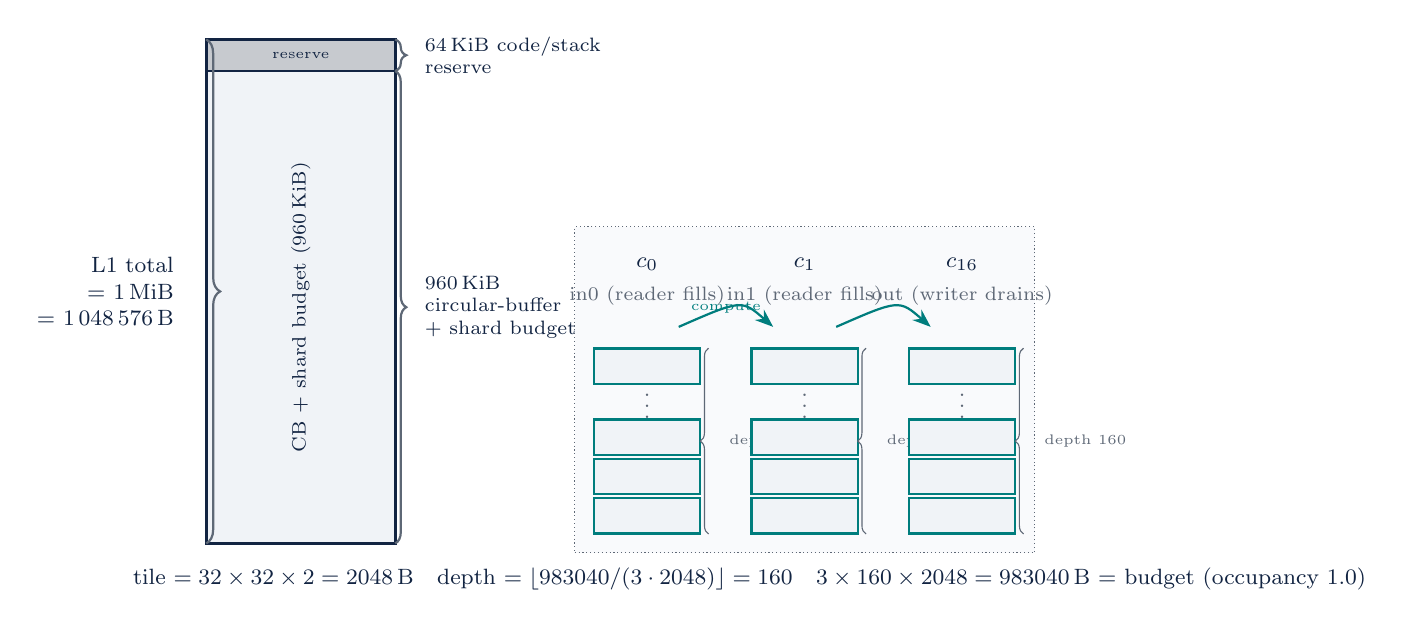
\begin{tikzpicture}[
      font=\small,
      tile/.style={draw=tensixteal, thick, fill=tensixlight,
                   minimum width=1.35cm, minimum height=4.5mm, inner sep=0pt},
      cblab/.style={font=\footnotesize\bfseries, text=tensixnavy},
      cbsub/.style={font=\scriptsize, text=tensixslate},
      note/.style={font=\footnotesize, text=tensixnavy, align=left},
    ]
    % ---- Left: per-core L1 bar, height proportional to bytes ----------------
    \def\barw{2.4} \def\barh{6.4}   % 6.4 cm = 1024 KiB; reserve = 64 KiB = 0.4 cm
    \coordinate (base) at (0,0);
    \fill[tensixlight] (base) rectangle ++(\barw,\barh);
    \fill[tensixslate!35] ($(base)+(0,\barh-0.4)$) rectangle ++(\barw,0.4);
    \draw[tensixnavy, very thick] (base) rectangle ++(\barw,\barh);
    \draw[tensixnavy, thick] ($(base)+(0,\barh-0.4)$) -- ++(\barw,0);
    \node[font=\tiny, text=tensixnavy] at ($(base)+(0.5*\barw,\barh-0.2)$) {reserve};
    \node[font=\scriptsize, rotate=90, text=tensixnavy]
      at ($(base)+(0.5*\barw,0.5*\barh-0.2)$) {CB + shard budget (960\,KiB)};

    % Brace left: total budget
    \draw[decorate, decoration={brace, amplitude=5pt}, thick, tensixslate]
      ($(base)+(0,\barh)$) -- (base)
      node[midway, left=8pt, align=right, font=\footnotesize, text=tensixnavy]
        {L1 total\\$=$ 1\,MiB\\$=$ 1\,048\,576\,B};
    % Braces right: reserve and CB/shard budget
    \draw[decorate, decoration={brace, amplitude=4pt}, thick, tensixslate]
      ($(base)+(\barw,\barh)$) -- ++(0,-0.4)
      node[midway, right=7pt, font=\scriptsize, text=tensixnavy, align=left]
        {64\,KiB code/stack\\reserve};
    \draw[decorate, decoration={brace, amplitude=4pt}, thick, tensixslate]
      ($(base)+(\barw,\barh-0.4)$) -- ($(base)+(\barw,0)$)
      node[midway, right=7pt, font=\scriptsize, text=tensixnavy, align=left]
        {960\,KiB\\circular-buffer\\+ shard budget};

    % ---- Right: the three circular buffers as tile queues --------------------
    \foreach \x/\idx/\role in {5.6/c_0/in0 (reader fills),
                               7.6/c_1/in1 (reader fills),
                               9.6/c_{16}/out (writer drains)} {
      \node[cblab] at (\x, 3.55) {$\idx$};
      \node[cbsub, align=center] at (\x, 3.15) {\role};
      \foreach \dy in {0, 0.5, 1.0} {
        \node[tile] at (\x, 0.35+\dy) {};
      }
      \node[font=\footnotesize, text=tensixslate] at (\x, 1.85) {$\vdots$};
      \node[tile] at (\x, 2.25) {};
      \draw[decorate, decoration={brace, amplitude=3pt}, thin, tensixslate]
        (\x+0.78, 0.12) -- (\x+0.78, 2.48)
        node[midway, right=4pt, font=\tiny, text=tensixslate] {depth 160};
    }
    % compute flow between buffers
    \draw[-Stealth, tensixteal, thick] (6.0, 2.75) .. controls (6.8, 3.1) .. (7.2, 2.75);
    \node[font=\tiny, text=tensixteal] at (6.6, 3.0) {compute};
    \draw[-Stealth, tensixteal, thick] (8.0, 2.75) .. controls (8.8, 3.1) .. (9.2, 2.75);

    % ---- Bottom: the arithmetic ------------------------------------------------
    \node[note] at (6.9, -0.45)
      {tile $= 32 \times 32 \times 2 = 2048$\,B\quad
       depth $= \lfloor 983040 / (3 \cdot 2048) \rfloor = 160$\quad
       $3 \times 160 \times 2048 = 983040$\,B $=$ budget (occupancy 1.0)};

    % background grouping for the CB region
    \begin{scope}[on background layer]
      \node[fit={($(5.6,0)+( -0.85,-0.05)$) ($(9.6,3.9)+(0.85,0.05)$)},
            draw=tensixslate, thin, densely dotted, fill=tensixlight!40,
            inner sep=2pt] {};
    \end{scope}
  \end{tikzpicture}
  \caption{Memory view of one modeled core. Left: the per-core L1 budget of
    \texttt{L1Model.h} --- 1\,MiB total minus a 64\,KiB code/stack reserve leaves
    the 960\,KiB circular-buffer + shard budget. Right: the default three-buffer
    pipeline ($c_0$ in0, $c_1$ in1, $c_{16}$ out) drawn as on-chip
    producer/consumer tile queues at depth 160; the three buffers consume exactly
    the budget ($983040$\,B, occupancy 1.0). Tile size 2048\,B is bf16 32x32.}
  \label{fig:theory-core-memory}
\end{figure}

\subsection{Operator fusion}

Without fusion, every operator boundary round-trips DRAM: RMSNorm reads the
activation from DRAM and writes the normalized intermediate back out, and the
following MatMul re-reads that same intermediate from DRAM (plus the weight) before
writing its output. Fusing the pair into one kernel keeps the intermediate resident
in L1 between the two stages --- the rmsnorm output never leaves the core that
produced it --- and erases both the intermediate DRAM write and the intermediate
DRAM re-read.

For the running example \texttt{rmsnorm\_matmul} (activation
$[1, 2048, 4096]$ bf16, weight $[4096, 12288]$ bf16) the intermediate has the same
shape as the activation, so it costs $1 \times 2048 \times 4096 \times 2 =
16\,777\,216$ bytes. That is exactly the figure the planner records in the plan
JSON as \texttt{estimated\_dram\_reads\_saved} (and
\texttt{estimated\_intermediate\_writes\_saved}): \textbf{16\,777\,216 bytes} each,
with the eliminated tensor counted on the fused op via the
\texttt{tensixflow.eliminated\_bytes} / \texttt{tensixflow.eliminated\_tensors}
annotations. Figure~\ref{fig:theory-fusion-dataflow} contrasts the two dataflows.

The fusion pass goes one step further on the full MLP chain
(\texttt{examples/mlp\_block.mlir}):
\[
  \text{rmsnorm} \to \text{matmul}(W_1) \to \text{add}(b_1) \to \text{gelu}
  \to \text{matmul}(W_2) \to \text{add}(\text{residual})
\]
is collapsed, link by link with a single-use guard at every intermediate, into a
single \texttt{tensixflow.fused\_mlp} kernel --- one kernel launch instead of six
operators, with all intermediates circulating in L1/registers rather than DRAM.%
\footnote{Grounding reference (inline per the citation-free contract):
  arXiv:2606.09879, \emph{Operator Fusion for LLM Inference on the Tensix
  Architecture} --- fuses RMSNorm with matmul in on-chip SRAM to cut DRAM
  read/write of intermediates, and distributes inputs/weights across the mesh via
  NoC row/column master-node multicast. The project's fixed 0.9875 correctness
  floor comes from the same paper's bf16-vs-fp32 context.}

\begin{figure}[t]
  \centering
  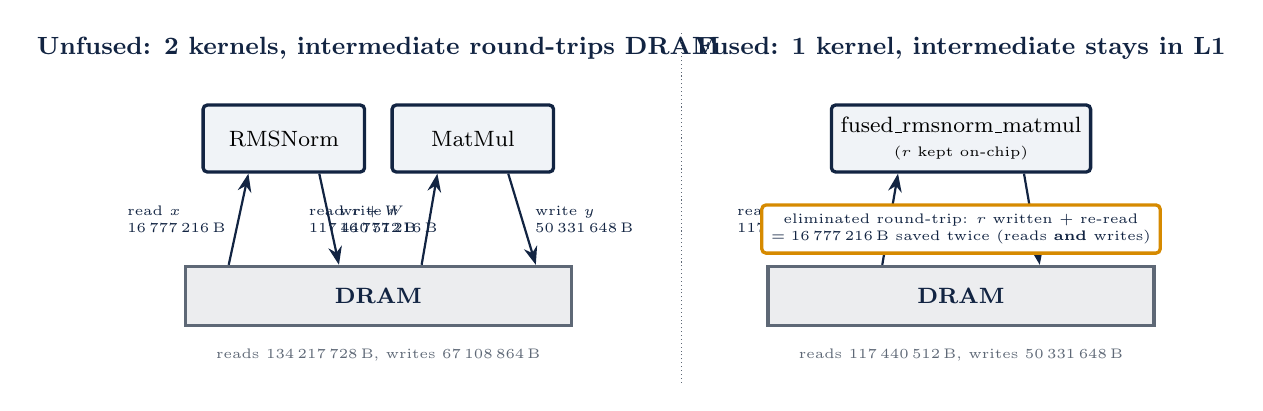
\begin{tikzpicture}[
      font=\small,
      kern/.style={draw=tensixnavy, very thick, fill=tensixlight,
                   rounded corners=1.5pt, minimum height=0.85cm,
                   minimum width=2.05cm, align=center, font=\footnotesize},
      dram/.style={draw=tensixslate, very thick, fill=tensixslate!12,
                   minimum height=0.75cm, minimum width=4.9cm, align=center,
                   font=\footnotesize\bfseries, text=tensixnavy},
      io/.style={-Stealth, thick, tensixnavy},
      saved/.style={-Stealth, thick, tensixamber, densely dashed},
      iolab/.style={font=\tiny, text=tensixnavy, align=left},
      paneltit/.style={font=\small\bfseries, text=tensixnavy},
    ]
  % ===================== UNFUSED =====================
  \node[paneltit] at (2.45, 3.35) {Unfused: 2 kernels, intermediate round-trips DRAM};
  \node[kern] (rn) at (1.25, 2.2) {RMSNorm};
  \node[kern] (mm) at (3.65, 2.2) {MatMul};
  \node[dram] (d1) at (2.45, 0.2) {DRAM};
  \draw[io] ($(d1.north)+(-1.9,0)$) -- ($(rn.south)+(-0.45,0)$)
    node[iolab, midway, left=1pt] {read $x$\\$16\,777\,216$\,B};
  \draw[io] ($(rn.south)+(0.45,0)$) -- ($(d1.north)+(-0.5,0)$)
    node[iolab, midway, right=0pt] {write $r$\\$16\,777\,216$\,B};
  \draw[io] ($(d1.north)+(0.55,0)$) -- ($(mm.south)+(-0.45,0)$)
    node[iolab, midway, left=1pt] {read $r + W$\\$117\,440\,512$\,B};
  \draw[io] ($(mm.south)+(0.45,0)$) -- ($(d1.north)+(2.0,0)$)
    node[iolab, midway, right=1pt] {write $y$\\$50\,331\,648$\,B};
  \node[font=\tiny, text=tensixslate, align=center] at (2.45, -0.55)
    {reads $134\,217\,728$\,B, writes $67\,108\,864$\,B};

  % ===================== FUSED =====================
  \node[paneltit] at (9.85, 3.35) {Fused: 1 kernel, intermediate stays in L1};
  \node[kern, minimum width=3.2cm] (fk) at (9.85, 2.2)
    {fused\_rmsnorm\_matmul\\[-1pt]{\tiny($r$ kept on-chip)}};
  \node[dram] (d2) at (9.85, 0.2) {DRAM};
  \draw[io] ($(d2.north)+(-1.0,0)$) -- ($(fk.south)+(-0.8,0)$)
    node[iolab, midway, left=1pt] {read $x + W$ once\\$117\,440\,512$\,B};
  \draw[io] ($(fk.south)+(0.8,0)$) -- ($(d2.north)+(1.0,0)$)
    node[iolab, midway, right=1pt] {write $y$ only\\$50\,331\,648$\,B};
  \node[font=\tiny, text=tensixslate, align=center] at (9.85, -0.55)
    {reads $117\,440\,512$\,B, writes $50\,331\,648$\,B};

  % elimination callout
  \node[draw=tensixamber, very thick, rounded corners=1.5pt, fill=white,
        font=\tiny, text=tensixnavy, align=center] at (9.85, 1.05)
    {eliminated round-trip: $r$ written + re-read\\ $= 16\,777\,216$\,B saved twice
     (reads \textbf{and} writes)};

  % separator
  \draw[tensixslate, thin, densely dotted] (6.3, -0.9) -- (6.3, 3.55);
  \end{tikzpicture}
  \caption{Unfused vs.\ fused dataflow for the running example. Unfused, the
    normalized intermediate $r$ ($16\,777\,216$\,B, same shape as the activation)
    is written to DRAM and re-read, adding one DRAM write and one DRAM read to the
    two-kernel execution. Fused, the intermediate stays in L1 between the stages:
    DRAM reads drop $134\,217\,728 \to 117\,440\,512$\,B and writes
    $67\,108\,864 \to 50\,331\,648$\,B --- the
    \texttt{estimated\_dram\_reads\_saved} $= 16\,777\,216$ figure recorded in
    \texttt{reports/rmsnorm\_matmul\_plan.json}. Byte figures are static analytic
    estimates from \texttt{docs/performance\_model.md}, not hardware measurements.}
  \label{fig:theory-fusion-dataflow}
\end{figure}

\subsection{NoC-aware sharding}

\texttt{-{}-tensixflow-plan-noc-sharding} maps the tensor shapes onto the 8x8 shard
grid and picks, tensor by tensor, how the data moves:

\begin{itemize}[nosep]
  \item \textbf{Activation: row-major sharding.} The leading (batch/M) dimension is
        row-major sharded across the grid's Y-cores, so each core row owns a
        contiguous band of rows and streams them tile by tile. The plan records
        this as \texttt{activation\_sharding: "row-major"}.
  \item \textbf{Weight: replicate or column-shard + multicast.} The weight planner
        compares the weight's footprint against the per-core circular-buffer budget
        of Figure~\ref{fig:theory-core-memory}. A weight that fits is
        \emph{replicated}: every core holds a full copy and multicast traffic is
        zero. A weight that does not fit is \emph{column-sharded} across the grid's
        X-cores and \emph{multicast} across the grid's rows via row master nodes,
        so it is moved once over the NoC rather than re-read from DRAM per core.
        The running example's weight ($[4096, 12288]$ bf16 $= 100\,663\,296$\,B
        $\gg$ 960\,KiB) takes the multicast path; the plan records
        \texttt{weight\_strategy: "multicast"}.
\end{itemize}

On top of the placement, the NoC traffic estimator produces a first-order static
account of both the unfused and the fused execution. For the running example it
reports unfused DRAM reads of
$16\,777\,216 + 16\,777\,216 + 100\,663\,296 = 134\,217\,728$ bytes
(activation $+$ intermediate $+$ weight) and unfused writes of
$16\,777\,216 + 50\,331\,648 = 67\,108\,864$ bytes (intermediate $+$ matmul
output), versus fused DRAM
reads $117\,440\,512$ bytes (activation + weight only, with the weight's
$100\,663\,296$ bytes counted once as NoC multicast) and writes $50\,331\,648$,
with the $16\,777\,216$-byte intermediate held L1-resident. These estimates are
also what the static performance model turns into the memory-vs-compute bound
classification; every figure is a shape-derived analytic estimate, never a measured
hardware number.

\subsection{Numerical validation theory}

The primary correctness metric is the Pearson correlation coefficient between the
simulator output vector $x$ and the golden output vector $y$:
\begin{equation}
  \mathrm{PCC}(x, y) \;=\;
  \frac{\sum_i (x_i - \bar{x})(y_i - \bar{y})}
       {\sqrt{\sum_i (x_i - \bar{x})^2}\;\sqrt{\sum_i (y_i - \bar{y})^2}},
  \label{eq:theory-pcc}
\end{equation}
with a \textbf{fixed correctness floor of 0.9875}: any run of either example graph
below the floor is a failure, and the floor is never lowered.%
\footnote{The floor and its context come from arXiv:2606.09879 (hardware bf16
  execution versus an fp32 reference, PCC kept above 98.75\%), the same grounding
  reference cited in Section~\ref{sec:theory}'s fusion subsection.}

The comparison is deliberately \emph{unequal-precision}: the simulator models the
bf16 spatial machine while the golden is fp32-exact, so Equation~\eqref{eq:theory-pcc}
measures a real quantity rather than an identity. Two effects of compiled execution
show up in the gap, and only in the gap:

\begin{enumerate}[nosep]
  \item \textbf{Precision cost.} The spatial machine rounds inputs to bf16, rounds
        every output tile back to bf16, and --- inside a fused kernel --- stores the
        intermediates between fused stages as bf16 in circular buffers
        (Figure~\ref{fig:theory-precision-flow}). Each round is a loss the
        fp32-exact golden never pays.
  \item \textbf{Tiled-execution cost.} Tile-by-tile accumulation adds partial sums
        in a different order than the composed whole-tensor evaluation of the
        golden, changing the rounding history even at fixed precision.
\end{enumerate}

If the golden also rounded its intermediates to bf16, the two paths would coincide
and PCC would collapse to 1.0, making any floor pass for nothing. The project
therefore keeps the golden fp32-exact and guards the bar with a layered
non-vacuity defense: a structural assertion that the golden's fused intermediates
are fp32 while the simulator output is bf16-representable, a bit-difference check
($\max_i |x_i - y_i| > 0$, i.e.\ PCC is strictly below 1.0), and an empirically
calibrated upper trip-wire above the measured good-case PCC. On the documented
seeds the measured minima are $\mathrm{PCC} = 0.99999316$ for
\texttt{rmsnorm\_matmul} and $\mathrm{PCC} = 0.99998885$ for \texttt{mlp\_block}
--- far above the 0.9875 floor, and strictly below 1.0, which is exactly the band
the rounding contract predicts.

\begin{figure}[t]
  \centering
  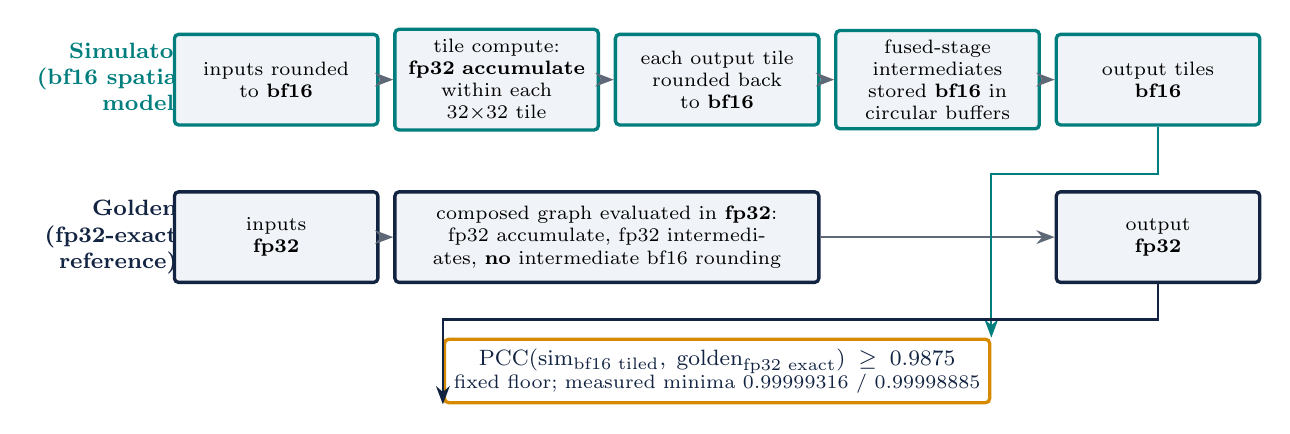
\begin{tikzpicture}[
      font=\footnotesize,
      simbox/.style={draw=tensixteal, very thick, fill=tensixlight,
                     rounded corners=1.5pt, align=center, font=\scriptsize,
                     text width=2.35cm, minimum height=1.15cm},
      goldbox/.style={draw=tensixnavy, very thick, fill=tensixlight,
                      rounded corners=1.5pt, align=center, font=\scriptsize,
                      text width=2.35cm, minimum height=1.15cm},
      flow/.style={-Stealth, thick, tensixslate},
      lanelab/.style={font=\footnotesize\bfseries, align=right},
    ]
  % ---- Simulator lane (bf16 spatial model) ----
  \node[lanelab, text=tensixteal] at (-0.4, 2.0) {Simulator\\(bf16 spatial\\model)};
  \node[simbox] (s1) at (1.7, 2.0) {inputs rounded\\to \textbf{bf16}};
  \node[simbox] (s2) at (4.5, 2.0) {tile compute:\\\textbf{fp32 accumulate}\\within each $32{\times}32$ tile};
  \node[simbox] (s3) at (7.3, 2.0) {each output tile\\rounded back\\to \textbf{bf16}};
  \node[simbox] (s4) at (10.1, 2.0) {fused-stage intermediates stored \textbf{bf16} in circular buffers};
  \node[simbox] (s5) at (12.9, 2.0) {output tiles\\\textbf{bf16}};
  \draw[flow] (s1) -- (s2); \draw[flow] (s2) -- (s3);
  \draw[flow] (s3) -- (s4); \draw[flow] (s4) -- (s5);

  % ---- Golden lane (fp32-exact) ----
  \node[lanelab, text=tensixnavy] at (-0.4, 0.0) {Golden\\(fp32-exact\\reference)};
  \node[goldbox] (g1) at (1.7, 0.0) {inputs\\\textbf{fp32}};
  \node[goldbox, text width=5.15cm] (g2) at (5.9, 0.0)
    {composed graph evaluated in \textbf{fp32}: fp32 accumulate, fp32 intermediates,
     \textbf{no} intermediate bf16 rounding};
  \node[goldbox] (g3) at (12.9, 0.0) {output\\\textbf{fp32}};
  \draw[flow] (g1) -- (g2); \draw[flow] (g2) -- (g3);

  % ---- Comparison ----
  \node[draw=tensixamber, very thick, rounded corners=1.5pt, fill=white,
        font=\footnotesize, text=tensixnavy, align=center] (cmp) at (7.3, -1.7)
    {$\mathrm{PCC}(\text{sim}_{\text{bf16 tiled}},\; \text{golden}_{\text{fp32 exact}})
      \;\geq\; 0.9875$\\[-1pt]{\scriptsize fixed floor; measured minima
      $0.99999316$ / $0.99998885$}};
  \draw[-Stealth, thick, tensixteal] (s5.south) -- ++(0,-0.6) -| (cmp.north east);
  \draw[-Stealth, thick, tensixnavy] (g3.south) -- ++(0,-0.45) -| (cmp.south west);
  \end{tikzpicture}
  \caption{Precision flow under the rounding contract. The simulator lane pays the
    bf16 spatial cost --- input rounding, fp32 accumulation within a tile, per-tile
    bf16 rounding, and bf16 circular-buffer intermediates between fused stages ---
    while the golden runs the composed graph fp32-exact throughout. The PCC between
    the two outputs therefore measures the real numerical cost of fusion plus tiled
    execution, rather than collapsing to a vacuous 1.0.}
  \label{fig:theory-precision-flow}
\end{figure}

\clearpage
% Lane WA — design decisions + deviations. Uses longtable/booktabs (preamble).
\section{Design Decisions}\label{sec:decisions}

TensixFlow was planned before any code was written, and the plan kept an explicit
decision register (drafts D1--D32 in the plan workspace) that was revised by three
rounds of adversarial review. Table~\ref{tab:decisions-register} records the
decisions that shaped the delivered system; Section~\ref{sec:decisions-deviations}
records the points where execution deliberately and documentedly deviated from the
plan text. The numerical and architectural background referenced in the register is
developed in Section~\ref{sec:theory}.

\subsection{Decision register}

{\small
\setlength{\tabcolsep}{4pt}
\begin{longtable}{@{}p{1.1cm}p{3.55cm}p{2.9cm}p{4.75cm}p{1.5cm}@{}}
\caption{Decision register. IDs are the plan's draft-decision identifiers.
  ``Adopted'' means the decision was made during planning and the delivered system
  implements it; revisions note the review round that forced them.}
\label{tab:decisions-register}\\
\toprule
\textbf{ID} & \textbf{Decision} & \textbf{Alternatives considered}
  & \textbf{Rationale} & \textbf{Status} \\
\midrule
\endfirsthead
\multicolumn{5}{@{}l}{\footnotesize\textit{Table \ref{tab:decisions-register}
  (decision register) continued}}\\
\toprule
\textbf{ID} & \textbf{Decision} & \textbf{Alternatives considered}
  & \textbf{Rationale} & \textbf{Status} \\
\midrule
\endhead
\midrule
\multicolumn{5}{r@{}}{\footnotesize\textit{continued on next page}}\\
\endfoot
\bottomrule
\endlastfoot

D1
& Self-contained, out-of-tree compiler: own \texttt{tensixflow} MLIR dialect and a
  full lowering pipeline living in this repository.
& Building in-tree inside Tenstorrent's tt-forge / tt-mlir repositories.
& The only way to make hardware-free progress: the standalone stack builds and
  tests on an ordinary CPU machine with the nix LLVM 20.1.8 toolchain, needs no
  Tenstorrent checkout, and keeps every artifact inspectable. Compatibility with
  the Tenstorrent stack is handled later as a TTIR emitter plus a prose mapping
  doc, not by living inside their tree.
& Adopted \\

D18
& Toolchain spike first: build the upstream \texttt{llvm-project}
  \texttt{mlir/examples/standalone} example under the new nix flake + devenv
  shell before writing any dialect code.
& Starting dialect work directly against the new environment.
& The devenv + MLIR wiring (\texttt{MLIR\_DIR}/\texttt{LLVM\_DIR}/tblgen paths)
  was explicitly UNVERIFIED at plan time. A throwaway spike proves the wiring
  empirically; had it failed, the environment approach would have been revisited
  before any dialect investment.
& Adopted; spike passed \\

D22
& Pipeline-registration probe: prove \texttt{registerAllPasses()} plus multi-pass
  composition with a 2-pass lit test before relying on the full seven-pass
  pipeline.
& Building the full pipeline first and debugging registration through it.
& The synthesized pipeline-registration syntax was UNVERIFIED at plan time; the
  2-pass probe isolates registration risk from pass-logic risk.
& Adopted; probe passed \\

D14 (execution)
& Numerical validation at the schedule-IR level: the functional simulator executes
  the schedule IR produced by \texttt{-{}-tensixflow-lower-to-ttkernel} over
  modeled circular buffers.
& Executing the generated kernels on a device (impossible: no device owned);
  interpreting the emitted C++ (out of scope).
& No Tenstorrent device exists in this project, so the generated
  reader/compute/writer/host sources are validated structurally only (golden
  FileCheck against current-API tokens + compile-only check) and are never
  executed. Keeping the numeric claim one level above the codegen artifact is what
  keeps the honesty disclaimer true.
& Adopted \\

D14 (rounding)
& Deliberate precision gap: simulator = bf16 spatial model (inputs bf16, fp32
  accumulate within a tile, per-tile bf16 rounding, bf16 circular-buffer
  intermediates); golden = fp32-exact reference. See
  Figure~\ref{fig:theory-precision-flow} and Eq.~\eqref{eq:theory-pcc}.
& Original contract --- golden also rounds per-op to bf16 (rejected in review
  round 1, P0); a hard-coded $0.9999$ upper guard (rejected in review round 2,
  R1).
& Revised per adversarial review so the PCC measures real divergence: the original
  contract collapsed PCC $\to 1.0$ and made the 0.9875 bar vacuous; the hard-coded
  upper guard was miscalibrated and would false-fail a correct implementation
  (good-case PCC exceeds it for single ops). The delivered contract makes
  PCC(simulator\textsubscript{bf16 tiled}, golden\textsubscript{fp32 exact}) the
  measured cost of fusion + tiled execution, with non-vacuity guarded by a
  structural dtype assertion, a bit-difference check, and an empirically calibrated
  trip-wire.
& Adopted after two review revisions \\

D4
& Exactly one modeled device: Wormhole n150 class, 8x8 grid, 32x32 tiles,
  bf16/fp32, HiFi4, with a modeled 1\,MiB L1 per core.
& A multi-device target matrix; using the literal silicon budget.
& A single target avoids premature generalization, and the modeled 1\,MiB is a
  documented, conservative, tunable constant: the literal n150 L1 per core is
  larger ($\approx$1.5\,MB), so the planner stays safely inside the real budget.
  Changing the one constant (and re-checking planner + model) is the supported way
  to target another budget.
& Adopted \\

D3
& Codegen targets the \emph{current} tt-metal API at \texttt{@df36cd6}: single
  \texttt{CreateKernel} with a \texttt{variant} of
  \texttt{DataMovementConfig}/\allowbreak\texttt{ComputeConfig}, \texttt{tt::CBIndex}
  circular buffers, \texttt{distributed::Enqueue*} mesh API.
& Emitting the legacy \texttt{EnqueueProgram} / per-role \texttt{CreateKernel}
  surface.
& \texttt{EnqueueProgram} no longer exists in the current \texttt{host\_api.hpp};
  it is kept only as a mapping note in \texttt{docs/tenstorrent\_mapping.md}. The
  golden structural tests assert current-API tokens only, and a legacy-API fixture
  is deliberately kept failing so the stub set cannot silently drift back to the
  legacy surface.
& Adopted \\

D15
& A single JSON schema as the plan/perf/viz contract, owned before the consumers
  and imported by all of them.
& Separate ad-hoc schemas per consumer (scheduler, perf model, report tool, HTML
  visualizer).
& One schema keeps the scheduler's plan, the perf model's figures, and the
  visualizer's sections from drifting apart. It is deliberately \emph{separate}
  from the MLIR-level schedule IR (D14), which is the codegen$\leftrightarrow$simulator
  contract; the two contracts serve different consumers.
& Adopted \\

D16
& Signature-only tt-metal stub headers as the substrate for the compile-only
  kernel check.
& Building real tt-metal (its runtime requires a device); skipping the compile
  check entirely.
& With no device, the stubs --- pinned to \texttt{@df36cd6} and covering both the
  host-API surface and the kernel-side intrinsics --- are the strongest available
  compile-time statement about the emitted code. The check asserts the presence of
  expected emitted symbols so it cannot pass vacuously, and a negative legacy-API
  fixture proves the stub set rejects the removed surface.
& Adopted \\

D17
& Shared L1-budget model: $\text{CB+shard budget} = L1_{\text{total}} -
  \text{reserve}$, $\text{CB\_bytes} = n_{\text{CB}} \times \text{depth} \times
  32 \times 32 \times 2$, defined once in \texttt{L1Model.h} and imported verbatim
  by the circular-buffer allocator and the perf model.
& Each component carrying its own copy of the constants.
& Single source of truth: the occupancy the perf model reports is exactly the
  budget the allocator actually planned against (Figure~\ref{fig:theory-core-memory}).
  Duplicating the constants would let the two silently disagree.
& Adopted \\

\end{longtable}
}

\subsection{Deviation register}\label{sec:decisions-deviations}

Four points where execution deviated from the literal plan text. Each deviation was
documented at the time it was taken; none of them loosened a verification gate.

{\small
\setlength{\tabcolsep}{4pt}
\begin{longtable}{@{}p{0.9cm}p{3.5cm}p{8.4cm}p{2.0cm}@{}}
\caption{Deviation register. ``T<number>'' refers to the plan's todo number whose
  acceptance prose was affected.}
\label{tab:decisions-deviation-register}\\
\toprule
\textbf{ID} & \textbf{Plan said} & \textbf{Deviation taken and why}
  & \textbf{Status} \\
\midrule
\endfirsthead
\multicolumn{4}{@{}l}{\footnotesize\textit{Table
  \ref{tab:decisions-deviation-register} (deviation register) continued}}\\
\toprule
\textbf{ID} & \textbf{Plan said} & \textbf{Deviation taken and why}
  & \textbf{Status} \\
\midrule
\endhead
\bottomrule
\endlastfoot

T37
& Acceptance prose invoked \texttt{-{}-emit-metalium \ldots -o <dir>} to write the
  generated project.
& A bare \texttt{-o <dir>} is impossible for an MLIR pass option:
  \texttt{MlirOptMain} owns the global \texttt{-o} output-file flag, and
  \texttt{PassOptions} options are parsed only out of the pass flag's value string.
  Implemented and documented as
  \texttt{-{}-tensixflow-emit-metalium=output-dir=<dir>} (recorded in the pass's
  TableGen description and the lit test header); acceptance was met in the
  deviated form.
& Documented deviation \\

T50
& Optional tt-mlir build + \texttt{ttmlir-opt} study, off the critical path.
& The heavy build (tt-mlir compiles a private 30--60\,min LLVM toolchain) was
  skipped on this box; the plan-sanctioned disjunctive OR branch was taken instead:
  \texttt{docs/ttmlir\_study.md} documents the skip reason and carries verbatim
  source-study snippets from tt-mlir's own test files at \texttt{@9f06802f}.
& Passed via OR branch \\

T55
& On-device branch: compile the generated kernels against real tt-metal, run them,
  and validate PCC $\geq 0.9875$ against the golden.
& Skipped: there is no \texttt{/dev/tenstorrent} on this machine, so the branch is
  gated out by design. Acceptance is covered by the disjunctive hardware harness,
  which passes via its explicit if/else no-device branch (bring-up dry-run +
  compile-only kernel check) --- the on-device branch was never silently replaced,
  only deferred.
& Skipped (gated); not failed \\

T60
& Submit the prepared upstream contribution as a CI-green PR (or patch + issue).
& Submission skipped per the explicit owner instruction ``DO NOT SUBMIT ANY PRS''.
  The contribution was implemented and verified locally (upstream pre-commit suite
  green, checks run against the current upstream main) and is committed to the
  repository's \texttt{upstream/} tree as a documentation-only artifact; no fork,
  push, PR, or issue was created.
& Documented only, per owner instruction \\

\end{longtable}
}

Two conventions close the register. Statuses are honest about what was \emph{not}
done: a gated skip is recorded as a skip, and a fallback branch is recorded as the
fallback, never as the primary outcome. And the honesty boundary from
Section~\ref{sec:theory} is preserved verbatim in every row: nothing in the
register upgrades ``structurally validated, never executed'' to ``executed'' or
``numerically verified''.

\clearpage
% =============================================================================
% Lane WB — Verification & honesty policy.
% Every claim grounded in: docs/architecture.md, docs/performance_model.md,
% scripts/hw_acceptance.sh, .omo/plans/tensixflow.md (guardrails),
% .omo/evidence/task-41-tensixflow.json, .omo/evidence/task-F3-tensixflow.log,
% .omo/start-work/ledger.jsonl. No external citations (contract: cite-free).
% =============================================================================
\section{Verification and Honesty Policy}\label{sec:policy}

TensixFlow's acceptance policy is built around one principle: \emph{two different
claims must never be conflated}. The first claim --- numerical correctness --- is
validated at the schedule-IR level by a functional simulator. The second claim ---
the emitted TT-Metalium kernel sources --- is validated structurally only, because
no Tenstorrent device exists anywhere in this campaign's loop. This section states
the honesty policy verbatim, describes the layered non-vacuity defense that keeps
the numeric bar from becoming meaningless, defines the disjunctive acceptance rule
for the hardware and upstream waves, and lists the scope guardrails that bound the
whole project.

\subsection{Honesty policy: generated kernels are structurally validated only}
\label{sec:policy-honesty}

The project's own documentation carries a disclaimer that this report quotes
verbatim rather than paraphrases, from \path{docs/architecture.md}
(\S\emph{Honesty disclaimer}):

\begin{quote}
``Nothing in this project executes the generated C++ kernels on hardware. There is
no Tenstorrent device in the loop, and no claim of on-device behavior anywhere.''

\smallskip
``In short: the schedule is numerically validated; the generated kernels are
structurally aligned and compile-checked. The two are different claims, and this
project keeps them separate on purpose.''
\end{quote}

Concretely, the generated kernels (\path{host.cpp}, \path{reader.cpp},
\path{compute.cpp}, \path{writer.cpp}) pass exactly two structural layers, both
executed by the test suite and never by prose:

\begin{enumerate}[leftmargin=1.6em]
  \item \textbf{Golden FileCheck patterns against the current tt-metal API}
    (pinned \texttt{@df36cd6}): the patterns assert current-API tokens --- the
    single \texttt{CreateKernel} with a \texttt{variant<ComputeConfig,\
    DataMovementConfig>}, \texttt{tt::CBIndex::c\_N} circular buffers, and the
    \texttt{distributed::Enqueue*} mesh API.
  \item \textbf{A compile-only \texttt{-fsyntax-only} check} of every generated
    kernel against signature-only tt-metal stub headers pinned to
    \texttt{@df36cd6}. The stubs carry no behavior; they exist so that an API
    drift becomes a compile error rather than a silent mismatch.
\end{enumerate}

The check is made non-vacuous by a deliberately failing negative fixture: a kernel
that calls the \emph{removed} legacy \texttt{EnqueueProgram} API must be rejected
by the stub set. The F3 hands-on QA run logged the pair explicitly: the current-API
baseline compiled, the legacy fixture failed with \texttt{EnqueueProgram}
undeclared (exit~1), and all four generated kernel files compiled
\texttt{-fsyntax-only} (\path{.omo/evidence/task-F3-tensixflow.log}, step~8).
Numeric correctness, in contrast, is asserted only at the schedule-IR level, as
detailed in Section~\ref{sec:policy-nonvacuity} and exercised end-to-end in
Section~\ref{sec:orchestration-finalwave}.

\textbf{Policy rule for numbers.} Every numeric claim in this report and in the
repository (PCC values, trip-wires, saved bytes, test counts) must originate from a
running test or harness invocation recorded in \path{.omo/evidence/}, never from
prose. This is the plan's own guardrail: ``No hand-waved correctness: every numeric
claim (PCC, bytes-saved) must come from a running test/harness, never prose.''

\subsection{Layered non-vacuity defense: keeping the PCC bar honest}
\label{sec:policy-nonvacuity}

A similarity metric is only meaningful if it can fail for the right reasons. The
similarity bar here --- Pearson correlation coefficient (PCC) between simulator
output and the NumPy golden --- could silently degenerate in two directions: a
\emph{corrupted} implementation that happens to stay above the floor, or a
\emph{vacuous} implementation where both sides compute identically so the metric
reads a meaningless perfect score. The campaign defends against both with a
layered design, and the layers are ordered from structural to empirical.

\paragraph{Rounding contract (why divergence is real).}
The two compared paths are \emph{deliberately} at different precision. The
functional simulator is the bf16 spatial model: inputs rounded to bf16, fp32
accumulation within a tile, each output tile rounded back to bf16, and fused
intermediates stored bf16 between stages. The golden reference is fp32-exact
throughout the composed graph, with no intermediate bf16 rounding. PCC between the
two therefore measures the real bf16-spatial-versus-exact cost of fusion plus tiled
execution --- and it structurally \emph{cannot} be identically~1.0.

\paragraph{Primary layer --- structural assertion + bit difference.}
Every harness run records three structural facts: the golden holds fused
intermediates in fp32, the simulator output is bf16, and the golden output dtype is
fp32 (fields \texttt{structural.*} in
\path{.omo/evidence/task-41-tensixflow.json}, true on all 16 runs). On top of that,
the harness asserts the bit-difference check
$\max|\text{sim}-\text{golden}| > 0$: if the two outputs were ever bit-identical
(the both-bf16-identical vacuous case), the run would fail deterministically. In
the recorded runs the gap is far from degenerate:
$\max|\text{sim}-\text{golden}|$ spans $2.77\times10^{-2}$ to
$4.13\times10^{-2}$ across all 16 runs of both targets
(\path{.omo/evidence/task-F3-tensixflow.log}, step~7).

\paragraph{Secondary layer --- empirically calibrated upper trip-wire.}
The upper band is \emph{not} a hard-coded constant. The trip-wire is calibrated
from the running implementation on the four documented seeds
(\texttt{0x20260727}, \texttt{0x5eed2026}, \texttt{0xc0ffee}, \texttt{0x1352777}):
take the measured good-case PCC and set the trip-wire strictly above it but
strictly below~1.0 --- in practice the midpoint between the good-case PCC
and~1.0. Hard-coding a value such as $0.9999$ was explicitly rejected: a clean
software bf16 model can exceed it, and the gate would false-fail correct code. As
recorded in the metrics JSON: for \texttt{rmsnorm\_matmul} the good-case PCC is
$0.9999940843$ and the trip-wire $0.9999970422$; for \texttt{mlp\_block},
$0.9999906926$ and $0.9999953463$. The lower bar $0.9875$ is a \textbf{fixed}
correctness floor: it is never lowered, and divergence is never injected to land
inside the band (\path{docs/performance_model.md}).

Table~\ref{tab:policy-nonvacuity} gives the full recorded picture, and
Figure~\ref{fig:policy-pcc-band} shows the pass band geometrically, including where
the two degenerate failure modes land.

\begin{table}[t]
  \centering
  \footnotesize
  \caption{Recorded PCC band per target (16 runs total: 2 targets $\times$ 2
    shapes $\times$ 4 seeds; source \texttt{.omo/evidence/task-41-tensixflow.json}).
    The trip-wire is the midpoint between the good-case PCC and 1.0, so it is
    recalibrated whenever the implementation's good case moves.}
  \label{tab:policy-nonvacuity}
  \begin{tabular}{@{}l r r r r@{}}
    \toprule
    Target & Measured PCC range & Good-case PCC & Trip-wire & Floor \\
    \midrule
    \texttt{rmsnorm\_matmul} & $0.999993159$--$0.999994084$ & $0.999994084$ & $0.999997042$ & $0.9875$ \\
    \texttt{mlp\_block}      & $0.999988845$--$0.999990693$ & $0.999990693$ & $0.999995346$ & $0.9875$ \\
    \bottomrule
  \end{tabular}
\end{table}

\begin{figure}[t]
  \centering
  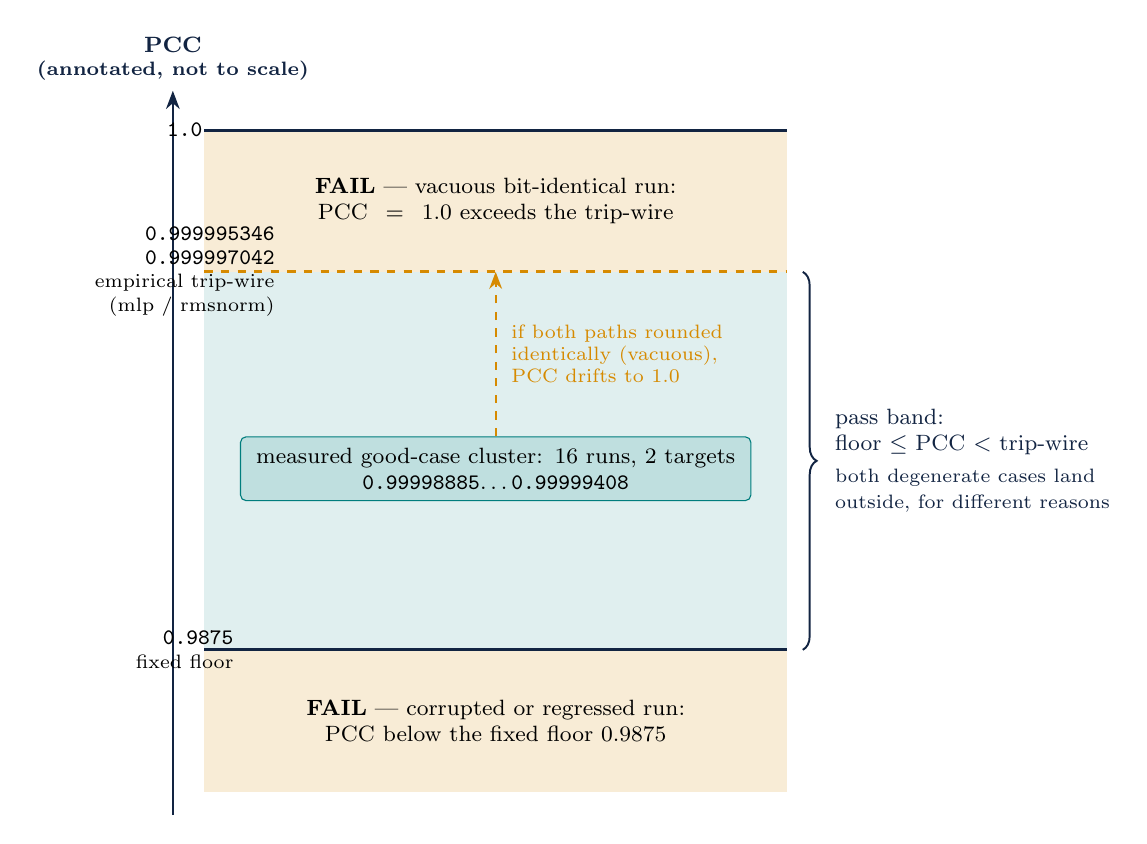
\begin{tikzpicture}[
    >=Stealth,
    zonefail/.style={fill=tensixamber!16},
    zonepass/.style={fill=tensixteal!12},
    boundary/.style={line width=1pt, tensixnavy},
    trip/.style={line width=1pt, tensixamber, dashed},
    vlab/.style={font=\footnotesize, align=right},
  ]
  % --- zone fills: x band from 0.4 to 7.8 ------------------------------------
  \fill[zonefail] (0.4,0.2) rectangle (7.8,2.0);
  \fill[zonepass] (0.4,2.0) rectangle (7.8,6.8);
  \fill[zonefail] (0.4,6.8) rectangle (7.8,8.6);
  % --- axis (annotated, NOT linearly scaled) ---------------------------------
  \draw[->, line width=0.8pt, tensixnavy] (0,-0.1) -- (0,9.1)
    node[above, font=\footnotesize\bfseries, align=center] {PCC\\[-1pt]\scriptsize(annotated, not to scale)};
  % --- boundaries + exact values ---------------------------------------------
  \draw[boundary] (0.4,2.0) -- (7.8,2.0);
  \node[vlab] at (0.15,2.0) {\texttt{0.9875}\\[-1pt]\scriptsize fixed floor};
  \draw[trip] (0.4,6.8) -- (7.8,6.8);
  \node[vlab] at (0.15,6.8) {\texttt{0.999995346}\\[-1pt]\texttt{0.999997042}\\[-1pt]\scriptsize empirical trip-wire\\[-1pt]\scriptsize(mlp / rmsnorm)};
  \draw[boundary] (0.4,8.6) -- (7.8,8.6);
  \node[vlab] at (0.15,8.6) {\texttt{1.0}};
  % --- zone texts --------------------------------------------------------------
  \node[font=\footnotesize, align=center, text width=6.6cm] at (4.1,1.1)
    {\textbf{FAIL} --- corrupted or regressed run:\\ PCC below the fixed floor $0.9875$};
  \node[font=\footnotesize, align=center, text width=6.6cm] at (4.1,7.7)
    {\textbf{FAIL} --- vacuous bit-identical run:\\ $\mathrm{PCC}=1.0$ exceeds the trip-wire};
  % --- measured cluster ---------------------------------------------------------
  \node[draw=tensixteal, fill=tensixteal!25, rounded corners=2pt,
        font=\footnotesize, align=center, text width=6.2cm, inner sep=4pt]
    (cluster) at (4.1,4.3)
    {measured good-case cluster: 16 runs, 2 targets\\
     \texttt{0.99998885}\ldots\texttt{0.99999408}};
  % --- vacuous drift arrow --------------------------------------------------------
  \draw[->, dashed, tensixamber, line width=0.7pt] (cluster.north) -- (4.1,6.8)
    node[midway, right=2pt, font=\scriptsize, align=left]
      {if both paths rounded\\ identically (vacuous),\\ PCC drifts to $1.0$};
  % --- pass-band brace ---------------------------------------------------------------
  \draw[decorate, decoration={brace, amplitude=5pt, mirror}, tensixnavy, line width=0.7pt]
    (8.0,2.0) -- (8.0,6.8)
    node[midway, right=8pt, font=\footnotesize, align=left]
      {pass band:\\ floor $\le$ PCC $<$ trip-wire\\[2pt]
       \scriptsize both degenerate cases land\\ \scriptsize outside, for different reasons};
  \end{tikzpicture}
  \caption{The non-vacuity pass band on the PCC metric. The corrupted-run failure
    mode (below the fixed floor $0.9875$) and the vacuous-run failure mode
    ($\mathrm{PCC}=1.0$, bit-identical outputs) sit on opposite sides of the pass
    band and are caught by different layers: the floor and the empirically
    calibrated trip-wire respectively, with the structural fp32-golden/bf16-simulator
    assertion and the $\max|\text{sim}-\text{golden}|>0$ check underneath both.
    Axis positions are schematic; all annotated values are exact, from
    \texttt{.omo/evidence/task-41-tensixflow.json}.}
  \label{fig:policy-pcc-band}
\end{figure}

The harness encodes each layer as an executable test, all green in the final
hands-on QA run (11/11 in \path{test_correctness.py}):
\path{test_pcc_above_floor},
\path{test_max_abs_diff_positive_not_bit_identical},
\path{test_pcc_below_empirical_tripwire},
\path{test_tripwire_calibrated_above_good_case}, and
\path{test_structural_fp32_golden_bf16_simulator}, each parametrized over
both targets.

\subsection{Disjunctive acceptance policy}
\label{sec:policy-disjunctive}

Two acceptance gates depend on resources the campaign does not control: a
Tenstorrent device (not owned) and an upstream maintainer's merge decision (not
owned). Both are therefore phrased \emph{disjunctively} --- each passes on a
documented fallback as well as on the full path --- with one strict structural
requirement on how the disjunction is written.

\paragraph{Hardware wave: explicit \texttt{if/else}, never \texttt{\&\&\ldots||}.}
The acceptance harness \path{scripts/hw_acceptance.sh} probes the device node and
runs exactly one branch:

\begin{lstlisting}[basicstyle=\ttfamily\scriptsize, frame=single, caption={Disjunctive hardware acceptance shape --- verbatim skeleton from \texttt{scripts/hw\_acceptance.sh} (\texttt{TT\_DEVICE\_PATH} defaults to \texttt{/dev/tenstorrent}).}, label={lst:policy-hwaccept}]
if [ -e "${TT_DEVICE_PATH}" ]; then
  # ON-DEVICE branch (todo 55): compile + run generated kernels,
  # validate PCC >= 0.9875 vs the NumPy golden.
  bash scripts/hw_run_on_device.sh
else
  # NO-DEVICE branch (todo 56): runbook dry-run + compile-only check.
  bash scripts/hw_bringup_dryrun.sh \
    && cmake --build build --target check-generated-kernels-compile
fi
\end{lstlisting}

The \texttt{if/else} is deliberate. An \texttt{on-device \&\&\ldots\ ||\
no-device} form would let a \emph{present-but-failing} device run fall through to
the passing no-device branch and be silently masked; with \texttt{if/else} exactly
one branch runs and the script's exit status is that branch's status, unmasked. The
on-device arm fails honestly even in absence of its entry point: if
\texttt{hw\_run\_on\_device.sh} is missing or non-executable the script exits~1
and refuses to fall through. On this campaign's CPU-only box the no-device arm is
the active one and did real work: bring-up dry-run exit~0 plus
\texttt{check-generated-kernels-compile} exit~0 (baseline compiles, legacy fixture
rejected, four generated kernels compile) --- see the final-wave QA in
Section~\ref{sec:orchestration-finalwave}. The on-device branch itself (todo~55)
was skipped and is recorded as such in the ledger, because no device is owned.

\paragraph{Upstream wave: submitted, never ``merged''.}
The upstream contribution gate accepts either an open pull request with the
\emph{contributor's own} checks green, or a prepared \path{0001-*.patch} plus an
issue URL. It never depends on the maintainers' CI and never claims a merge, since
neither is owned by this campaign. In the event, the campaign owner issued an
explicit do-not-subscribe/do-not-submit override, so todo~T60 landed as
\emph{documented-only}: the scouted target, the contribution, and the submission
procedure are committed under \path{upstream/}, and the ledger records
``T60 skipped --- submission process documented only.''

\subsection{Scope guardrails as policy}
\label{sec:policy-guardrails}

The plan's ``Must NOT have'' list is enforced as acceptance policy, not as advice:
each stretch surface has a binding guardrail and an executable or auditable check.
Table~\ref{tab:policy-guardrails} reproduces them together with how each was
verified during the campaign (final-wave evidence cited where applicable; see
Section~\ref{sec:orchestration-finalwave}).

\begin{table}[t]
  \centering
  \footnotesize
  \caption{Scope guardrails binding the campaign, and the check that enforced each.}
  \label{tab:policy-guardrails}
  \begin{tabular}{@{}p{2.7cm} p{6.1cm} p{5.2cm}@{}}
    \toprule
    Surface & Guardrail (binding) & Enforced / verified by \\
    \midrule
    Python DSL & Thin MLIR-text builder only; \emph{no} tracing JIT, no AST
      introspection & Canonicalized-IR equivalence test vs the handwritten inputs
      (ignoring SSA names); F4 import audit: no \texttt{ast}/\texttt{inspect} \\
    TT-MLIR compat & TTIR \emph{emitter} only; the other four dialects are prose
      mappings & \texttt{--tensixflow-emit-ttir} lit test; mapping doc covers
      TTIR/TTNN/D2M/TTKernel/TTMetal in prose \\
    Remote-box script & \texttt{bash -n} syntax check + docs only; never live
      provisioning, no cloud spend & \texttt{bash -n scripts/remote-box.sh}
      exit~0; script never executed; pricing prose dated ``as-of 2026-07-21'' \\
    Benchmarks & Timing loops, \emph{not} a framework & No benchmark-framework
      dependency (\texttt{find\_package(benchmark)} absent); each binary prints an
      explicit static-estimate disclaimer \\
    HTML visualizer & Static, offline, zero external references & Playwright load
      with all network requests aborted: 0 requests, 0 console errors, 6/6 section
      anchors; 0 \texttt{http(s)} occurrences in the source \\
    Owner constraints & nix/devenv shell binding the whole build; no NVIDIA GPU;
      no PR submission (T60 documented-only) & Every gate runs under
      \texttt{nix develop}; F3 probes: no \path{/dev/tenstorrent}, no NVIDIA in
      \texttt{lspci}; F4 audit: nothing submitted/forked/merged \\
    \bottomrule
  \end{tabular}
\end{table}

Two further guardrails shape everything downstream: exactly \emph{one} modeled
device (Wormhole n150-class: 8$\times$8 grid, 32$\times$32 tiles, bf16/fp32,
1~MiB modeled L1 per core) --- no multi-target support --- and no NVIDIA/CUDA path
at all, since this is a spatial-accelerator compiler and the campaign owns no
NVIDIA GPU. Both were re-audited adversarially by the F4 scope-fidelity review
(repo-wide greps for \texttt{cuda|nvidia}, \texttt{grayskull|blackhole|n300}, and
multi-device tokens came back clean except a single sanctioned
absence-statement in a test docstring). Hardware specifics are covered in
Section~\ref{sec:hardware}.

\clearpage
% =============================================================================
% 04_orchestration.tex — lane WB, completed by integrator WI.
% Sources: .omo/plans/tensixflow.md (waves, todos, final verification wave),
%          .omo/boulder.json (works.tensixflow-f194c7b3.task_sessions and
%            session_ids; per-task elapsed_ms fields),
%          .omo/start-work/ledger.jsonl (task events, adversarial classes),
%          .omo/evidence/ (task-* files, F3 QA log, W0 report evidence).
% Citation-free per the BUILDING.md contract.
% =============================================================================
\section{Orchestration}\label{sec:orchestration}

This section describes how the campaign was actually run, which is as much a
deliverable as the compiler itself: a single orchestrator session drove every
todo through a fixed execution loop, eleven parallel waves with two sanctioned
skips, and a four-reviewer final verification wave. Every timing and count
quoted here traces to \path{.omo/boulder.json}, \path{.omo/start-work/
ledger.jsonl}, or \path{.omo/evidence/}; none is reconstructed from memory.
The policy that bounded the work (honesty, non-vacuity, disjunctive acceptance,
scope guardrails) is in Section~\ref{sec:policy}.

\subsection{Execution model}

The campaign ran as a closed loop over the plan's 60 todos
(Figure~\ref{fig:orch-execution-loop}). The loop's state is not prose: the plan
file \path{.omo/plans/tensixflow.md} is the single source of truth for waves,
todos, and agent-executable acceptance criteria, and \path{.omo/boulder.json}
mirrors it as machine state (active work ID, per-todo status, session IDs, and
per-task \texttt{elapsed\_ms} timings). Each todo was decomposed into a lane
assignment, delegated to a subagent, and accepted back only through an
independent verification gate.

\begin{figure}[t]
  \centering
  \resizebox{\textwidth}{!}{%
  \begin{tikzpicture}[
      font=\small,
      box/.style={draw=tensixnavy, very thick, fill=tensixlight,
                  rounded corners=2pt, align=center, inner sep=4pt,
                  minimum width=3.1cm, minimum height=1.2cm, font=\footnotesize},
      gbox/.style={draw=tensixamber, very thick, fill=tensixamber!12,
                   rounded corners=2pt, align=center, inner sep=4pt,
                   minimum width=3.2cm, minimum height=1.2cm, font=\footnotesize},
      okbox/.style={draw=tensixteal, very thick, fill=tensixteal!12,
                    rounded corners=2pt, align=center, inner sep=4pt,
                    minimum width=3.1cm, minimum height=1.2cm, font=\footnotesize},
      gate/.style={draw=tensixamber, very thick, fill=tensixamber!12,
                   diamond, aspect=1.5, align=center, inner sep=3pt,
                   font=\footnotesize},
      arr/.style={-{Stealth[length=2.4mm]}, tensixnavy, line width=0.9pt},
      blk/.style={-{Stealth[length=2.4mm]}, tensixamber, line width=0.9pt},
      lab/.style={font=\scriptsize, text=tensixnavy, align=center},
    ]
    % ---- top row: plan -> boulder state -> decompose --------------------
    \node[box] (plan) at (0,0)
      {\textbf{plan}\\[-1pt]\scriptsize \path{.omo/plans/tensixflow.md}\\[-1pt]
       \scriptsize waves, todos, acceptance criteria};
    \node[box] (state) at (5.4,0)
      {\textbf{boulder state}\\[-1pt]\scriptsize \path{.omo/boulder.json}\\[-1pt]
       \scriptsize per-todo status + session IDs};
    \node[box] (decomp) at (10.8,0)
      {\textbf{decompose to lanes}\\[-1pt]
       \scriptsize wave $\to$ todos by difficulty category};
    \draw[arr] (plan) -- (state);
    \draw[arr] (state) -- (decomp);
    % ---- right column: delegate -> DoneClaim ----------------------------
    \node[box] (delegate) at (10.8,-2.7)
      {\textbf{delegate to subagents}\\[-1pt]
       \scriptsize Sisyphus-Junior workers by category\\[-1pt]
       \scriptsize (quick / deep / writing / low);\\[-1pt]
       \scriptsize oracle reviewers: read-only audits};
    \node[box] (done) at (10.8,-5.3)
      {\textbf{DoneClaim}\\[-1pt]
       \scriptsize changed files + tests + risks};
    \draw[arr] (decomp) -- (delegate);
    \draw[arr] (delegate) -- (done);
    % ---- gate -------------------------------------------------------------
    \node[gate] (av) at (5.4,-5.3)
      {\textbf{AdversarialVerify}\\[-1pt] \scriptsize independent re-run};
    \draw[arr] (done) -- (av);
    % ---- ledger ------------------------------------------------------------
    \node[okbox] (ledger) at (0,-5.3)
      {\textbf{ledger + checkbox flip}\\[-1pt]
       \scriptsize \path{ledger.jsonl} event appended,\\[-1pt]
       \scriptsize todo checkbox in plan};
    \draw[arr] (av) -- (ledger)
      node[midway, above=2pt, lab, text=tensixteal] {only \texttt{confirmed} passes};
    % ---- rework loop (blocking verdicts) -----------------------------------
    \draw[blk] (av.south) -- ++(0,-0.8) -| (delegate.east)
      node[pos=0.9, right=2pt, align=left, font=\scriptsize, text=tensixamber]
        {\texttt{false-positive} / \texttt{needs-fix} /\\[-1pt]
         \texttt{needs-human-review} all block};
    % ---- close the loop -----------------------------------------------------
    \draw[arr] (ledger) -- (plan)
      node[midway, left=2pt, lab] {next todo};
  \end{tikzpicture}}%
  \caption{The campaign execution loop. Each todo moves plan $\to$ boulder
    state $\to$ lane decomposition $\to$ subagent delegation, returns a
    \texttt{DoneClaim}, and is accepted only when an independent
    \texttt{AdversarialVerify} run re-confirms it; only the verdict
    \texttt{confirmed} appends a \texttt{ledger.jsonl} event and flips the
    plan's checkbox. The three blocking verdicts route the todo back to
    delegation for rework. Structure from \texttt{.omo/start-work/ledger.jsonl}
    and \texttt{.omo/boulder.json}.}
  \label{fig:orch-execution-loop}
\end{figure}

Two properties make the loop trustworthy rather than ceremonial. First, every
verification is a re-run, not a re-read: the orchestrator independently
executed each todo's acceptance commands (for example, \texttt{check-tensixflow},
\texttt{ctest}, \texttt{pytest}, and the full lowering pipeline) rather than
trusting the worker's summary. Second, every task-completed ledger event
carries an \emph{adversarial-class} map: the same nine trigger-mapped QA
classes, assessed per task. The classes are malformed input, prompt injection,
cancel/resume, stale state, dirty worktree, hung/long commands, flaky tests,
misleading success output, and repeated interruptions; each event records
either a concrete probe (``probed: \ldots'') or an explicit
``not-applicable'' with the reason. The probes are real work, not labels: the
toolchain spike probed stale nix state and a dirty worktree, the first lit test
carried a deliberate wrong-CHECK negative proof, the CI workflow was grepped
for forbidden GPU/device tokens, and every early task verified that malformed
input produced a clean diagnostic rather than a crash (see
\path{.omo/evidence/task-1-tensixflow.log} through
\path{.omo/evidence/task-7-tensixflow.txt}).

\subsection{Wave plan}

The 60 todos were executed as eleven parallel waves
(Figure~\ref{fig:orch-wave-dag}). The critical spine is W1 (environment and
skeleton, the gating uncertainty) through W7 (simulator, correctness, perf
model, visualizer, benchmarks, and docs). Four side lanes hang off the spine:
W8 (the Python DSL) may begin once W2's dialect lands and integrates after W7;
W9 (TT-MLIR compatibility) and W10 (the conditional hardware path) both wait on
W6's codegen; W11 (the upstream contribution) waits on W9's familiarity. The
Final Wave F1--F4 runs after all todos and gates the whole campaign.

\begin{figure}[t]
  \centering
  \resizebox{\textwidth}{!}{%
  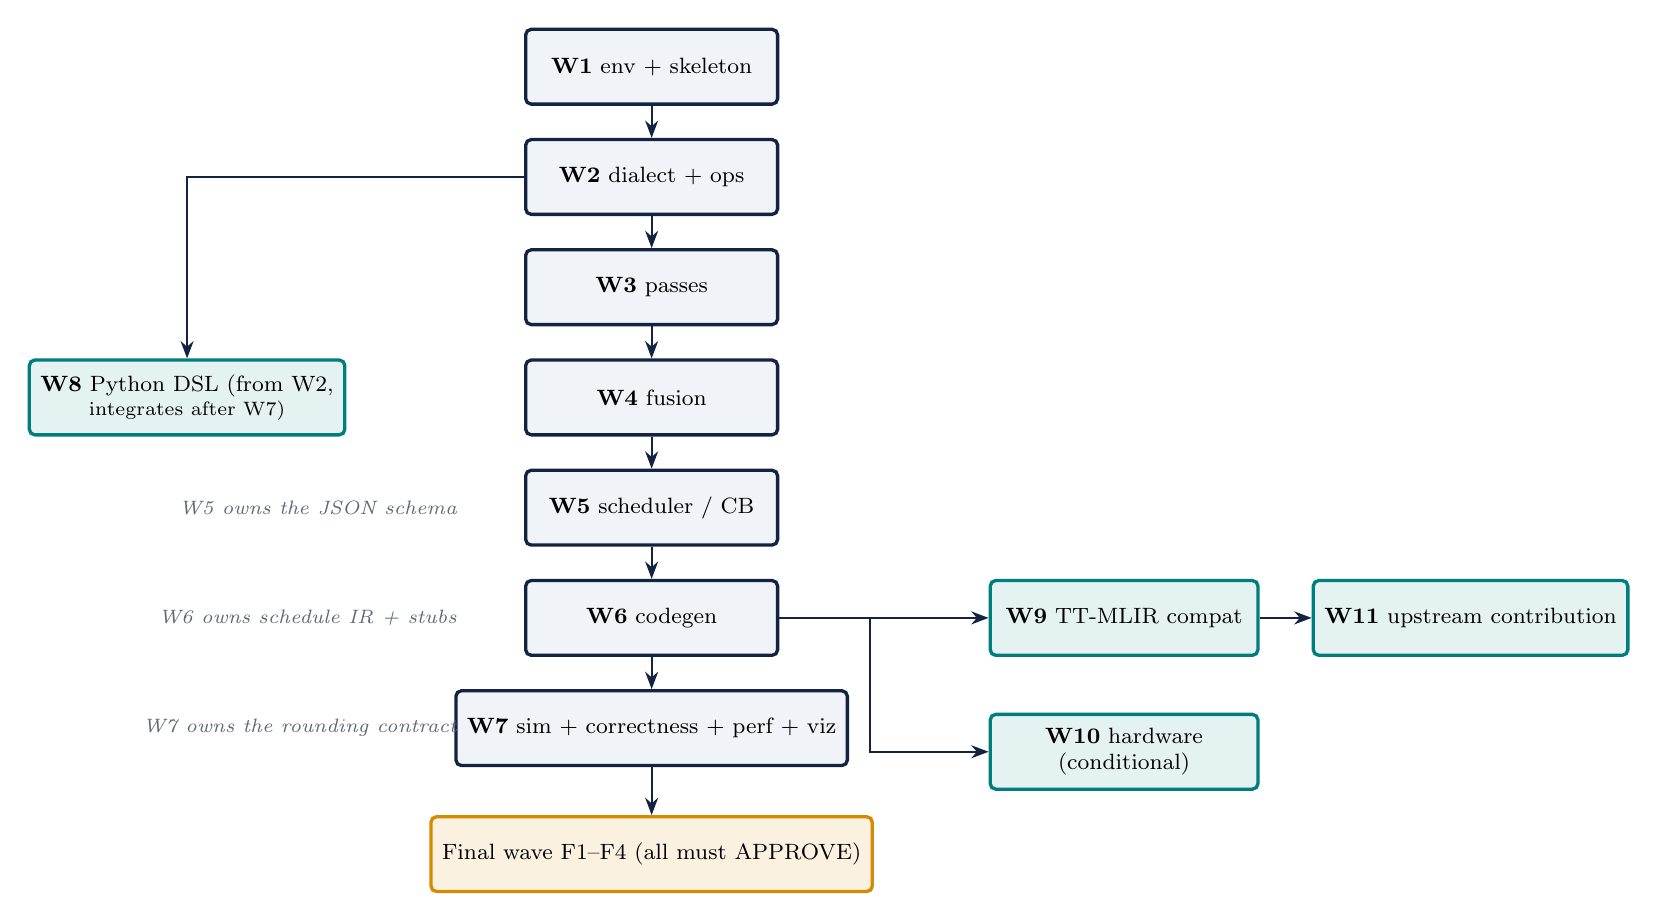
\begin{tikzpicture}[
      font=\small,
      wave/.style={draw=tensixnavy, very thick, fill=tensixlight,
                   rounded corners=2pt, align=center, inner sep=4pt,
                   minimum width=3.2cm, minimum height=0.95cm, font=\footnotesize},
      side/.style={draw=tensixteal, very thick, fill=tensixteal!10,
                   rounded corners=2pt, align=center, inner sep=4pt,
                   minimum width=3.4cm, minimum height=0.95cm, font=\footnotesize},
      fin/.style={draw=tensixamber, very thick, fill=tensixamber!12,
                  rounded corners=2pt, align=center, inner sep=4pt,
                  minimum width=5.2cm, minimum height=0.95cm, font=\footnotesize},
      tag/.style={font=\scriptsize\itshape, tensixslate, align=right},
      arr/.style={-{Stealth[length=2.2mm]}, tensixnavy, line width=0.8pt},
    ]
    % ---- critical spine ----------------------------------------------------
    \node[wave] (w1) at (0,7.6) {\textbf{W1} env + skeleton};
    \node[wave] (w2) at (0,6.2) {\textbf{W2} dialect + ops};
    \node[wave] (w3) at (0,4.8) {\textbf{W3} passes};
    \node[wave] (w4) at (0,3.4) {\textbf{W4} fusion};
    \node[wave] (w5) at (0,2.0) {\textbf{W5} scheduler / CB};
    \node[wave] (w6) at (0,0.6) {\textbf{W6} codegen};
    \node[wave] (w7) at (0,-0.8) {\textbf{W7} sim + correctness + perf + viz};
    \node[fin]  (fin) at (0,-2.4) {Final wave F1--F4 (all must APPROVE)};
    \draw[arr] (w1) -- (w2); \draw[arr] (w2) -- (w3);
    \draw[arr] (w3) -- (w4); \draw[arr] (w4) -- (w5);
    \draw[arr] (w5) -- (w6); \draw[arr] (w6) -- (w7);
    \draw[arr] (w7) -- (fin);
    % ---- side lanes -----------------------------------------------------------
    \node[side] (w8) at (-5.9,3.4) {\textbf{W8} Python DSL (from W2,\\[-1pt] \scriptsize integrates after W7)};
    \node[side] (w9) at (6.0,0.6) {\textbf{W9} TT-MLIR compat};
    \node[side] (w10) at (6.0,-1.1) {\textbf{W10} hardware \\(conditional)};
    \node[side] (w11) at (10.4,0.6) {\textbf{W11} upstream contribution};
    \draw[arr] (w2.west) -| (w8.north);
    \draw[arr] (w6.east) -- (w9.west);
    \draw[arr] (w6.east) -- ++(1.15,0) |- (w10.west);
    \draw[arr] (w9.east) -- (w11.west);
    % ---- cross-cutting contracts ----------------------------------------------
    \node[tag, anchor=east] at (-2.35,2.0) {W5 owns the JSON schema};
    \node[tag, anchor=east] at (-2.35,0.6) {W6 owns schedule IR + stubs};
    \node[tag, anchor=east] at (-2.35,-0.8) {W7 owns the rounding contract};
  \end{tikzpicture}}%
  \caption{The eleven-wave dependency DAG plus the final verification wave.
    The W1--W7 spine is the critical path; W8 starts from W2 and integrates
    after W7, W9 and W10 wait on W6, and W11 waits on W9. Three cross-cutting
    contracts are owned one wave each: W5 owns the plan/perf/viz JSON schema,
    W6 owns the schedule IR and the signature-only stub headers, and W7 owns
    the     bf16-simulator / fp32-golden rounding contract (Section
    \ref{sec:policy-nonvacuity}). Dependency matrix from
    \texttt{.omo/plans/tensixflow.md}.}
  \label{fig:orch-wave-dag}
\end{figure}

The wave plan carried three cross-cutting contracts that were decided once and
imported by every downstream consumer, never duplicated (Section
\ref{sec:policy}): W5 owns the plan/perf/viz JSON schema, W6 owns the MLIR
schedule IR (the codegen$\leftrightarrow$simulator contract) together with the
signature-only tt-metal stub headers pinned at \texttt{@df36cd6}, and W7 owns
the rounding contract that makes the PCC bar non-vacuous. Two todos were
plan-sanctioned skips rather than failures: T55 (on-device branch) because no
device is owned, covered by the disjunctive hardware acceptance
(Section~\ref{sec:policy-disjunctive}), and T60 (submit) because the owner
issued an explicit do-not-submit override; both are recorded as skips in the
ledger and produced no commits.

\subsection{Scale and cadence}

Per-task elapsed times were tracked in \path{.omo/boulder.json} as
\texttt{elapsed\_ms} fields. Table~\ref{tab:orch-timing} lists the notable
ones. The honest caveat on the headline number bears repeating in prose: the
176-hour campaign figure is wall-clock time from the first plan-approved state
to the final wave, so it includes idle time and human-wait time (the upstream
scout at 11h16m, for example, was the elapsed span of a long-running session,
not 11 hours of continuous compute). The per-task figures are the reliable
signal: even the heaviest implementation todos (T1, T12, T30, T39, T59)
measured in minutes to a few hours of wall-clock each.

\begin{longtable}{@{}p{1.0cm}p{6.2cm}p{3.3cm}p{4.4cm}@{}}
  \caption{Notable per-task elapsed wall-clock times from
    \texttt{.omo/boulder.json} (\texttt{elapsed\_ms} fields, converted).
    \texttt{T<number>} refers to the plan todo.}
  \label{tab:orch-timing}\\
  \toprule
  \textbf{Todo} & \textbf{Task} & \textbf{Elapsed} & \textbf{Note} \\
  \midrule
  \endfirsthead
  \multicolumn{4}{@{}l}{\small\itshape Table \thetable{} (continued)}\\
  \toprule
  \textbf{Todo} & \textbf{Task} & \textbf{Elapsed} & \textbf{Note} \\
  \midrule
  \endhead
  \bottomrule
  \endfoot
  T1 & Toolchain spike: nix flake + devenv on \texttt{llvmPackages\_20} &
    23\,m\,54\,s & Gating uncertainty; proved the env wiring first \\
  T12 & Consolidated shape-inference + verifier test suite &
    13\,m\,6\,s & Wave 2 \\[-1pt]
  T30 & \texttt{plan-noc-sharding} + \texttt{allocate-circular-buffers}
    passes + plan report & 10\,m\,44\,s & Wave 5; first consumer of the JSON
    schema \\
  T39 & Functional tile simulator over circular buffers &
    15\,m\,29\,s & Wave 7; executes the schedule IR \\
  T58 & Scout a concrete small upstream contribution &
    11\,h\,16\,m & Longest single task (repo reconnaissance) \\
  T59 & Implement the contribution per upstream style + tests &
    3\,h\,17\,m & Wave 11; \texttt{upstream/} artifact \\
  \midrule
  Campaign & Full plan-to-final-wave wall-clock &
    176\,h\,22\,m\,13\,s &
    \emph{includes idle / human-wait time, not pure compute} \\
  \bottomrule
\end{longtable}

Three repository counts, all measured by direct command on this box, anchor the
``one commit per todo, one evidence file per task'' claim:

\begin{itemize}[nosep]
  \item \texttt{git rev-list --count HEAD} returns \textbf{58} commits: one
        conventional commit per implemented todo, each leaving the tree green.
        The 60-todo plan minus the two sanctioned skips (T55, T60) is exactly
        58, and \texttt{git log --oneline} spot-checks the style, e.g.\
        \texttt{feat(upstream): implement contribution per upstream style +
        tests}, \texttt{test(hw): disjunctive hardware acceptance harness},
        \texttt{feat(sim): functional tile simulator over circular buffers}.
  \item \texttt{ls .omo/evidence | grep -c task-} returns \textbf{64}
        evidence files: every implemented todo 1--59 (excluding the two skips)
        has one, T41 and T43 additionally keep a metrics JSON and a rendered
        HTML, the F3 QA log and its two screenshots are archived, and the
        report pipeline's own evidence files live there too.
  \item \texttt{wc -l < .omo/start-work/ledger.jsonl} returns \textbf{68}
        lines: the work-started event, one task-completed or task-skipped event
        per todo, four wave-complete summaries, and four final-wave-verdict
        events (Section~\ref{sec:orchestration-finalwave}).
\end{itemize}

\subsection{Final verification wave}\label{sec:orchestration-finalwave}

After all todos landed, four independent read-only oracle reviewers ran in
parallel and each returned APPROVE (Table~\ref{tab:orch-finalwave}). Each
reviewer's session ID is recorded in \path{.omo/boulder.json} under
\texttt{works.tensixflow-f194c7b3.session\_ids}, and each verdict is logged in
\path{.omo/start-work/ledger.jsonl} as a \texttt{final-wave-verdict} event.
The wave was read-only by guarantee: \texttt{git status} after the wave showed
only untracked \path{.omo/} evidence, and zero product files were modified by
reviewers.

\begin{table}[t]
  \centering
  \footnotesize
  \caption{Final verification wave: four independent read-only oracle
    reviewers, all APPROVE. Session IDs are from
    \texttt{.omo/boulder.json} \texttt{works.tensixflow-f194c7b3.session\_ids};
    the four \texttt{final-wave-verdict} events are in
    \texttt{.omo/start-work/ledger.jsonl}.}
  \label{tab:orch-finalwave}
  \begin{tabular}{@{}p{0.5cm}p{2.0cm}p{4.6cm}p{5.6cm}c@{}}
    \toprule
    \textbf{ID} & \textbf{Reviewer role} & \textbf{Session ID} & \textbf{Read-only verification} & \textbf{Verdict} \\
    \midrule
    F1 & Plan compliance audit &
      \texttt{\scriptsize ses\_0361ca41cffeQDZJY0cmSiTjsD} &
      Re-runs every todo's acceptance command: \texttt{check-tensixflow}
      (25 = 24 passed + 1 unsupported), \texttt{ctest} (11/11),
      \texttt{pytest} (89 passed), and the full lowering pipeline on both
      examples (rc=0, 6 files each) &
      \textbf{APPROVE} \\
    F2 & Code quality review &
      \texttt{\scriptsize ses\_0361c328dffeo2zvLAMhPVZbkc} &
      Malformed/truncated IR and malformed JSON produce clean diagnostics,
      never crashes; codegen emits the current tt-metal API only (grep for
      \texttt{EnqueueProgram} emission sites is zero); stubs signature-only
      pinned \texttt{@df36cd6}; ruff advisory pass &
      \textbf{APPROVE} \\
    F3 & Hands-on QA &
      \texttt{\scriptsize ses\_0361bc016ffeEqisSH5eTHC1S0} &
      Build $\to$ lit $\to$ ctest $\to$ pytest $\to$ pipeline on both
      examples $\to$ report regeneration (byte-identical) $\to$
      simulator-vs-golden harness (PCC $\ge$ 0.9875 both targets, non-vacuity
      holds) $\to$ \texttt{scripts/hw\_acceptance.sh} no-device branch $\to$
      network-blocked Playwright render (0 requests, 6/6 anchors) &
      \textbf{APPROVE} \\
    F4 & Scope fidelity &
      \texttt{\scriptsize ses\_0361b41aaffe7faVAxXHZYusN4} &
      Adversarial greps for \texttt{cuda|nvidia}, multi-device tokens, and
      submitted/merged-PR claims; op-zoo and \texttt{L1Model.h} constants
      audits; DSL import audit (no \texttt{ast}/\texttt{inspect}/\texttt{torch});
      upstream tree audit (nothing submitted, forked, or merged) &
      \textbf{APPROVE} \\
    \bottomrule
  \end{tabular}
\end{table}

The campaign's direct session
(\texttt{ses\_0780d1f23ffeVINbwloM0T7ZwW}) is the orchestrator session shared
across the boulder works; the four F-wave reviewers are the appended sessions
listed above. The F3 verdict is also preserved as evidence:
\path{.omo/evidence/task-F3-tensixflow.log} (with the two
\texttt{task-F3-screenshot-*.png} renders) records every step's exit code, the
captured PCC values for both targets, and the byte-identical report
regeneration. The F1--F4 approvals are the acceptance events the plan's final
verification wave requires.

One honest sentence on this document: this report is itself a follow-up
deliverable, written and compiled \emph{after} plan completion by a worker
outside the boulder loop, using an ephemeral
\texttt{nix shell nixpkgs\#texlive.combined.scheme-full} toolchain
(\texttt{report/BUILDING.md}) that resolved against the same pinned nixpkgs
rev without modifying the project flake, and its commit is therefore not
counted among the 58 implementation commits of the campaign.

\clearpage
% =============================================================================
% 05_hardware.tex — lane WC
% Sources: lib/tensixflow/Scheduler/L1Model.h, scripts/hw_probe.sh,
%          scripts/hw_bringup_dryrun.sh, scripts/hw_acceptance.sh,
%          .github/workflows/ci-hardware.yml, docs/hardware_path.md
% =============================================================================
\section{Hardware}\label{sec:hardware}

TensixFlow targets a modeled Tenstorrent Wormhole n150-class spatial
accelerator. The development box is CPU-only: \emph{no Tenstorrent device is
owned}, and nothing in the MVP touches hardware. This section documents the
device model the scheduler reasons about, the always-available no-device
validation, and the gated path that opens if a real n150 ever appears.

\subsection{The modeled device}

The device model lives in a single header,
\texttt{lib/tensixflow/Scheduler/L1Model.h}, which is the declared
\emph{single source of truth} for the per-core L1 budget: the circular-buffer
allocator and the static performance model import these constants verbatim
and are forbidden from duplicating them. The exact constants are reproduced
in Table~\ref{tab:hardware-device-spec}.

\begin{table}[htbp]
  \centering
  \caption{Modeled device specification. Constants are the exact values from
  \texttt{lib/tensixflow/Scheduler/L1Model.h}; the remaining rows are stated
  in \texttt{docs/hardware\_path.md} and \texttt{scripts/hw\_bringup\_dryrun.sh}.}
  \label{tab:hardware-device-spec}
  \begin{tabular}{@{}lp{4.0cm}p{4.6cm}@{}}
    \toprule
    \textbf{Parameter} & \textbf{Value} & \textbf{Grounding} \\
    \midrule
    Device class & Wormhole n150-class, single part & README, \texttt{L1Model.h} header \\
    Core grid & $8 \times 8$ Tensix grid (64 cores) & \texttt{L1Model.h} header comment \\
    Tile shape & $32 \times 32$ elements & \texttt{kTileBytes} definition \\
    Data formats & bf16 (storage), fp32 (accumulate) & \texttt{L1Model.h} header comment \\
    Math fidelity & \texttt{MathFidelity::HiFi4} & \texttt{docs/hardware\_path.md}, Step 1 \\
    \texttt{kL1TotalBytes} & $1024 \times 1024 = 1{,}048{,}576$ B (1 MiB/core) & \texttt{L1Model.h} \\
    \texttt{kL1ReserveBytes} & $64 \times 1024 = 65{,}536$ B (64 KiB, code/stack) & \texttt{L1Model.h} \\
    \texttt{kCBShardBudget} & \texttt{kL1TotalBytes} $-$ \texttt{kL1ReserveBytes} $= 983{,}040$ B (960 KiB) & \texttt{L1Model.h} \\
    \texttt{kTileBytes} & $32 \times 32 \times 2 = 2{,}048$ B & \texttt{L1Model.h} \\
    \bottomrule
  \end{tabular}
\end{table}

The modeled L1 per core is \textbf{conservative by design}: the literal
Wormhole n150 L1 is larger (about 1.5 MB), but TensixFlow models 1 MiB and
documents the caveat directly in the header comment. Every plan produced by
the sharding and CB-allocation passes is therefore provably within budget on
the real part if it fits the model.

\subsection{The per-core L1 budget model}

Figure~\ref{fig:hardware-l1-budget} renders the budget arithmetic exactly as
the constants define it: tt-metal addresses memory by $(x, y, \text{local L1
address})$, and each core's L1 is carved into a 64 KiB reserve (kernel code
and stack) plus the 960 KiB the planner may spend on circular buffers and
tensor shards. The circular-buffer sizing formula, in bytes, is
\begin{equation}
  \text{bytes}(\mathrm{CB}) = n_{\mathrm{CB}} \times \text{depth} \times 2048,
  \label{eq:hardware-cb-sizing}
\end{equation}
i.e.\ the number of buffers times the depth in 32$\times$32 tiles times
\texttt{kTileBytes} $= 2048$ B. The committed plan
\texttt{reports/rmsnorm\_matmul\_plan.json} instantiates this for the fused
RMSNorm+MatMul kernel: three CBs (\texttt{c\_0}, \texttt{c\_1}, \texttt{c\_16},
the tt-metal \texttt{tt::CBIndex} convention for in0/in1/out) at depth 160
tiles each, so $3 \times 160 \times 2048 = 983{,}040$ B --- exactly the
960 KiB \texttt{kCBShardBudget}, fully consumed.

\begin{figure}[htbp]
  \centering
  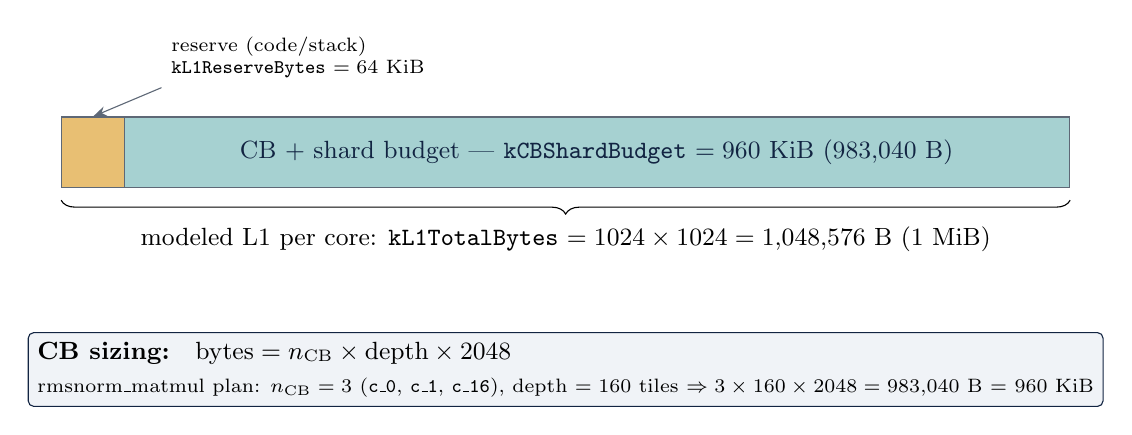
\begin{tikzpicture}[
      font=\small,
      seg/.style={draw=tensixslate, minimum height=0.9cm, anchor=west},
    ]
    % Total bar: 1024 KiB mapped to 12.8 cm (0.0125 cm per KiB)
    \node[seg, fill=tensixlight, minimum width=12.8cm] (total) at (0,0) {};
    % Reserve segment: 64 KiB -> 0.8 cm
    \node[seg, fill=tensixamber!55, minimum width=0.8cm] (reserve) at (0,0) {};
    % CB + shard budget segment: 960 KiB -> 12.0 cm
    \node[seg, fill=tensixteal!35, minimum width=12.0cm] (budget) at (0.8,0) {};
    % Reserve label with pointer (segment too narrow for inline text)
    \node[font=\scriptsize, align=left] (reslabel) at ($(reserve.north)+(2.6,0.75)$)
      {reserve (code/stack)\\ \texttt{kL1ReserveBytes} $= 64$ KiB};
    \draw[-{Stealth}, tensixslate] (reslabel.south west) -- (reserve.north);
    % Budget label inside the bar
    \node[font=\small, tensixnavy] at ($(budget.west)+(6.0,0)$)
      {CB + shard budget --- \texttt{kCBShardBudget} $= 960$ KiB ($983{,}040$ B)};
    % Brace under the whole bar: total
    \draw[decorate, decoration={brace, amplitude=5pt, mirror}]
      ($(total.south west)+(0,-0.15)$) -- ($(total.south east)+(0,-0.15)$)
      node[midway, below=6pt]
        {modeled L1 per core: \texttt{kL1TotalBytes} $= 1024 \times 1024 = 1{,}048{,}576$ B (1 MiB)};
    % CB sizing formula + worked example
    \node[draw=tensixnavy, fill=tensixlight, rounded corners=2pt,
          align=left, font=\small] at ($(total.south)+(0,-2.3)$)
      {\textbf{CB sizing:}\quad $\text{bytes} = n_{\mathrm{CB}} \times \text{depth} \times 2048$ \\[1pt]
       \scriptsize rmsnorm\_matmul plan: $n_{\mathrm{CB}}=3$ (\texttt{c\_0}, \texttt{c\_1}, \texttt{c\_16}),
       depth $=160$ tiles $\Rightarrow 3 \times 160 \times 2048 = 983{,}040$ B $=$ 960 KiB};
  \end{tikzpicture}
  \caption{Per-core L1 budget of the modeled Wormhole n150-class device, per
  \texttt{L1Model.h}: a 64 KiB reserve carved out of the 1 MiB total leaves the
  960 KiB circular-buffer/shard budget the planner spends, together with the CB
  sizing formula and the fused RMSNorm+MatMul working point from
  \texttt{reports/rmsnorm\_matmul\_plan.json}.}
  \label{fig:hardware-l1-budget}
\end{figure}

\subsection{Bring-up runbook (five validated steps)}

\texttt{scripts/hw\_bringup\_dryrun.sh} is the always-available half of the
hardware acceptance: it \emph{prints} the validated bring-up runbook (grounded
in tt-metal \texttt{INSTALLING.md} at the pinned revision \texttt{@df36cd6}),
probes \texttt{/dev/tenstorrent}, and always exits 0 --- a dry-run, not a
probe gate. Its five steps, summarized, are Table~\ref{tab:hardware-bringup}.

\begin{table}[htbp]
  \centering
  \caption{The five validated bring-up steps printed by
  \texttt{scripts/hw\_bringup\_dryrun.sh} for a Wormhole n150 box, from zero
  to a running generated kernel project.}
  \label{tab:hardware-bringup}
  \begin{tabular}{@{}lp{9.6cm}@{}}
    \toprule
    \textbf{Step} & \textbf{Summary (as the script prints it)} \\
    \midrule
    1. Obtain/access an n150 & Shell access to a Linux box with a Wormhole n150 seated (PCIe); the modeled target: $8\times8$ Tensix grid, $32\times32$ tiles, bf16. \\
    2. KMD + host tools & TT-Installer (\texttt{install.sh} v2.1.0, no container runtime): installs TT-KMD ($\ge$ v2.8.0), \texttt{tt-smi}, \texttt{tt-flash}. Once the KMD loads, \texttt{/dev/tenstorrent} exists --- the probe target the whole acceptance keys on. \\
    3. Build tt-metal with runtime & Clone \texttt{tt-metal}, \texttt{git checkout df36cd6}, run \texttt{./build\_metal.sh}. The runtime (host API + device dispatch) is required to enqueue kernels; TensixFlow's stub headers are only for the no-device structural check. \\
    4. Flash firmware & Flash before first use: TT-Installer drives \texttt{tt-flash}; Wormhole boards pair with \texttt{fw\_pack-19.8.1.fwbundle} (firmware v19.8.1). Verify card, FW version, and health with \texttt{tt-smi -s}. \\
    5. Run the generated project & Build \texttt{kernels/generated/fused\_rmsnorm\_matmul/} (host/reader/compute/writer.cpp) against the \emph{real} tt-metal, enqueue via \texttt{distributed::EnqueueMeshWorkload}, read back, and validate PCC $\ge 0.9875$ against the NumPy golden --- the same bar as the simulator harness. \\
    \bottomrule
  \end{tabular}
\end{table}

\subsection{Device / no-device acceptance}\label{sec:hardware-acceptance}

The hardware wave is accepted \emph{disjunctively}: either a run on a real
device with PCC $\ge 0.9875$ against the golden, or the validated no-device
substitute (bring-up runbook + compile-only kernel check + hardware-gated
CI). The disjunction is wired in \texttt{scripts/hw\_acceptance.sh} as an
\textbf{explicit if/else, never \texttt{\&\&\ldots||}}:

\begin{lstlisting}[language=bash]
if [ -e "${TT_DEVICE_PATH}" ]; then          # default: /dev/tenstorrent
  # ON-DEVICE branch: compile + run + PCC >= 0.9875 vs the golden.
  # Only this arm runs on a device box; a failure is never masked.
  bash scripts/hw_run_on_device.sh
else
  # NO-DEVICE branch: runbook dry-run + compile-only kernel check.
  bash scripts/hw_bringup_dryrun.sh && \
    cmake --build build --target check-generated-kernels-compile
fi
\end{lstlisting}

The \texttt{\&\&\ldots||} spelling would be unsafe: in
\texttt{on-device \&\& run || no-device}, a device that is \emph{present but
failing} would fall through to the passing no-device branch and its failure
would be masked. With \texttt{if/else} exactly one branch runs and the
script's exit status is that branch's status, unmasked; the harness also
fail-honestly exits nonzero if the on-device arm is reached without its entry
point (\texttt{scripts/hw\_run\_on\_device.sh}) present.

\paragraph{The no-device branch does real work.}
It is not a no-op. First, the dry-run runbook exits 0. Second,
\texttt{check-generated-kernels-compile} (mechanics in
Section~\ref{sec:software-stubs}) asserts three things: the current-API
baseline kernel compiles \texttt{-fsyntax-only} against the stubs, the legacy
fixture referencing the removed symbol \texttt{EnqueueProgram} is
\emph{rejected} with a diagnostic naming that symbol, and all four generated
kernel files (\texttt{host.cpp}, \texttt{reader.cpp}, \texttt{compute.cpp},
\texttt{writer.cpp}) compile. A typo in any generated kernel fails this
branch honestly.

\paragraph{The hardware-gated CI job.}
\texttt{.github/workflows/ci-hardware.yml} adds a single \texttt{on-device}
job, gated \textbf{twice} so it can never run on a deviceless box:
\begin{enumerate}[nosep]
  \item \emph{Label/dispatch gate (job-level \texttt{if}):} the PR must carry
        the \texttt{hardware.present} label, or the run must be an explicit
        \texttt{workflow\_dispatch} manual override.
  \item \emph{Runner gate (\texttt{runs-on}):}
        \texttt{[self-hosted, tenstorrent, wormhole-n150]} --- only a
        self-hosted runner tagged as carrying the hardware can pick the job
        up; GitHub-hosted runners never match.
\end{enumerate}
When both hold, the job first asserts \texttt{/dev/tenstorrent} exists and
exits 1 on absence --- a gated job that lands on a deviceless runner is a
misconfiguration that must fail honestly, not silently pass --- and then runs
the on-device entry point, failing loudly while that script does not yet
exist. In short: \emph{a skipped-on-device is never a silent pass.} The
ordinary CPU-only CI (Section~\ref{sec:deployment-ci}) is untouched and runs
on every push.

\clearpage
% =============================================================================
% 06_software.tex — lane WC
% Sources: tree layout, include/tensixflow/*.td, lib/tensixflow/**, tools/*,
%          kernels/handwritten_baselines/check_kernels_compile.sh,
%          python/tensixflow/**, test/, benchmarks/
% =============================================================================
\section{Software}\label{sec:software}

TensixFlow is a from-scratch C++/MLIR compiler stack: a custom
\texttt{tensixflow} dialect with tensor-level and fused ops, a
tile-level \emph{schedule IR}, seven lowering passes, a TT-Metalium-style
kernel emitter, a functional tile simulator, a static performance model with
an offline HTML visualizer, and a Python DSL plus a NumPy golden/correctness
harness. Everything builds and runs on a CPU-only box.

\subsection{Architecture}\label{sec:software-architecture}

Figure~\ref{fig:software-architecture} is the system map. The spine is
\texttt{tensixflow-opt}: hand-written MLIR (or MLIR text emitted by the
Python DSL) runs through five lowering passes, ending in the schedule IR.
That IR is the pivot: the emitter turns it into generated TT-Metalium-style
kernel projects (validated \emph{structurally only}), while the functional
tile simulator executes it directly (validated \emph{numerically} against an
fp32-exact NumPy golden). A side track exports the plan as JSON, runs the
static performance model, and renders the self-contained HTML report; a
compat track emits TTIR-shaped text.

\begin{figure}[htbp]
  \centering
  \resizebox{\textwidth}{!}{%
  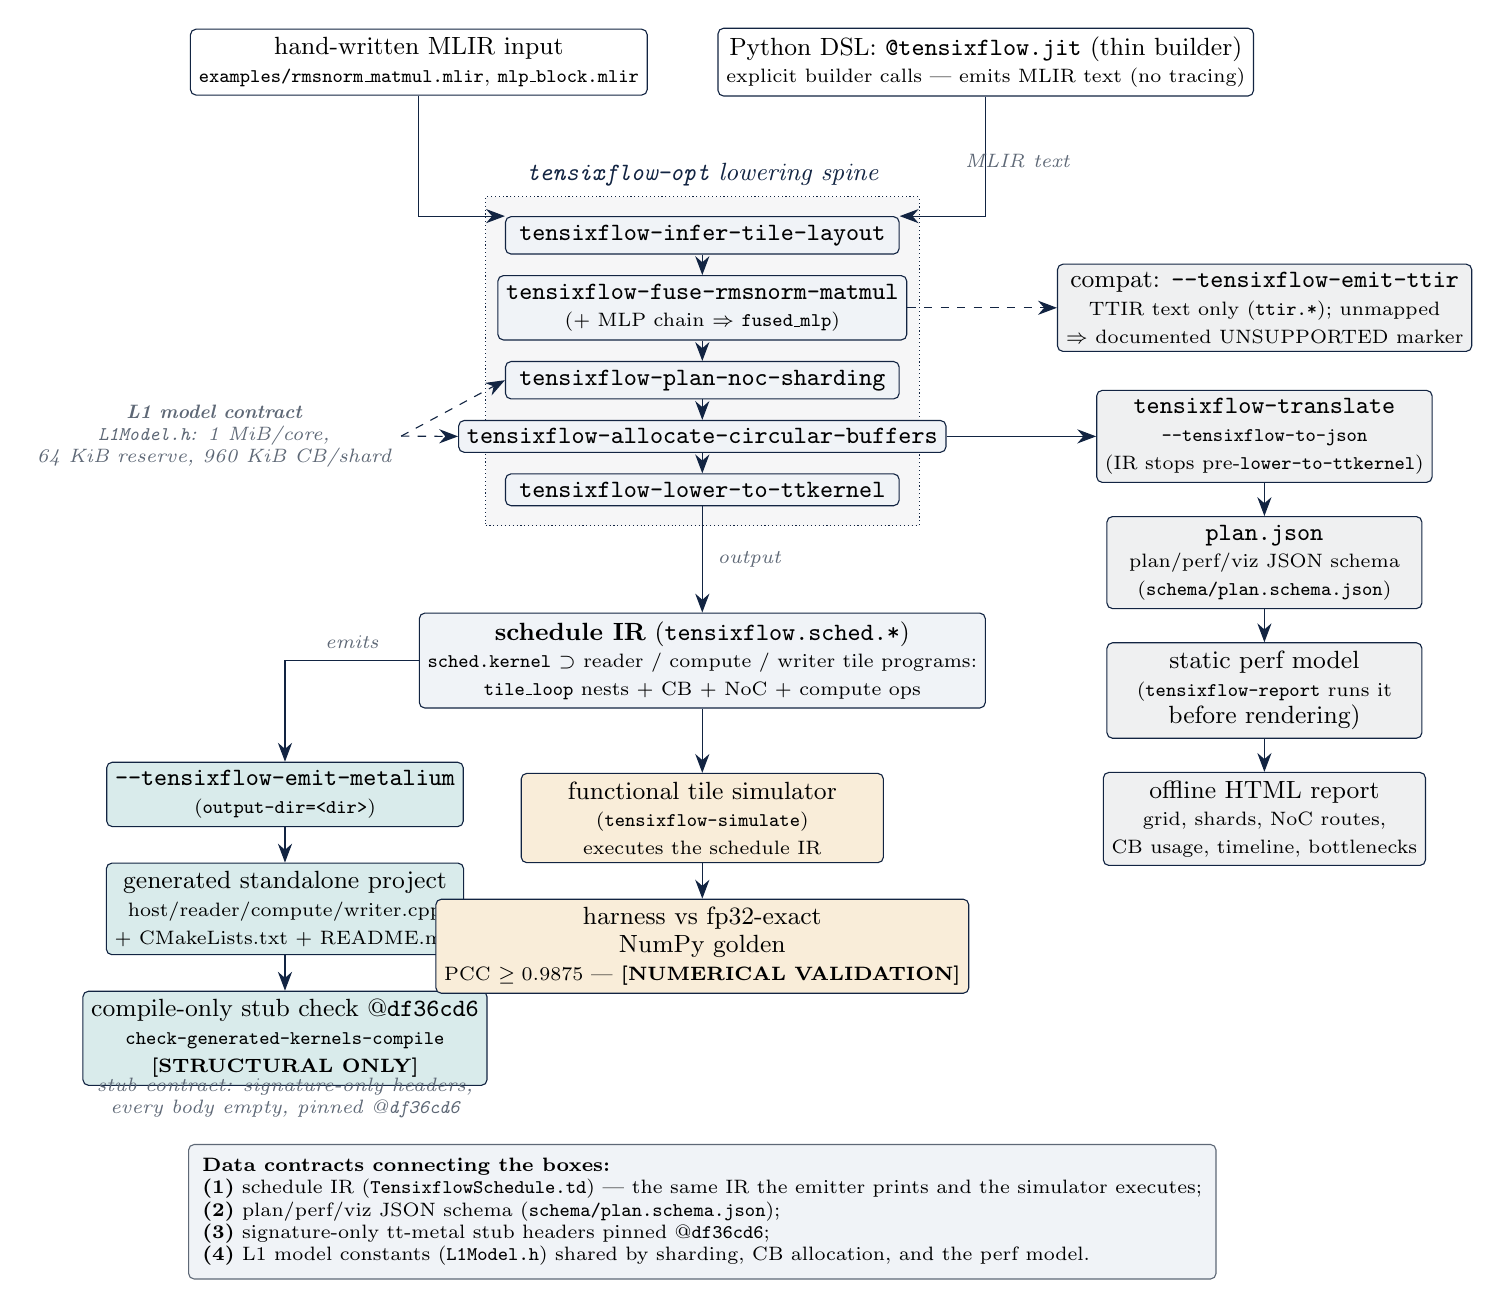
\begin{tikzpicture}[
      box/.style={draw=tensixnavy, rounded corners=2pt, align=center,
                  font=\small, inner sep=3pt, fill=white},
      pass/.style={box, fill=tensixlight, minimum width=6.4cm, font=\small},
      outA/.style={box, fill=tensixteal!15, minimum width=4.4cm},
      outB/.style={box, fill=tensixamber!15, minimum width=4.6cm},
      side/.style={box, fill=tensixslate!10, minimum width=4.0cm},
      tag/.style={font=\scriptsize\itshape, tensixslate},
      arr/.style={-{Stealth[length=2.4mm]}, tensixnavy},
    ]
    % ---- inputs -------------------------------------------------------------
    \node[box, minimum width=5.2cm] (mlir) at (-3.6,0)
      {hand-written MLIR input\\[-1pt]
       \scriptsize\texttt{examples/rmsnorm\_matmul.mlir}, \texttt{mlp\_block.mlir}};
    \node[box, minimum width=5.6cm] (dsl) at (3.6,0)
      {Python DSL: \texttt{@tensixflow.jit} (thin builder)\\[-1pt]
       \scriptsize explicit builder calls --- emits MLIR text (no tracing)};

    % ---- pass spine ----------------------------------------------------------
    \node[pass, minimum width=5.0cm] (p1) at (0,-2.2) {\texttt{tensixflow-infer-tile-layout}};
    \node[pass, minimum width=5.0cm, below=0.26cm of p1] (p2)
      {\texttt{tensixflow-fuse-rmsnorm-matmul}\\[-1pt]
       \scriptsize (+ MLP chain $\Rightarrow$ \texttt{fused\_mlp})};
    \node[pass, minimum width=5.0cm, below=0.26cm of p2] (p3) {\texttt{tensixflow-plan-noc-sharding}};
    \node[pass, minimum width=5.0cm, below=0.26cm of p3] (p4) {\texttt{tensixflow-allocate-circular-buffers}};
    \node[pass, minimum width=5.0cm, below=0.26cm of p4] (p5) {\texttt{tensixflow-lower-to-ttkernel}};
    \begin{scope}[on background layer]
      \node[fit=(p1)(p5), draw=tensixnavy, densely dotted, fill=tensixnavy!4,
            inner sep=7pt] (pipebox) {};
    \end{scope}
    \node[tag, tensixnavy, font=\small\itshape, anchor=south] at (pipebox.north)
      {\texttt{tensixflow-opt} lowering spine};
    \draw[arr] (mlir.south) |- (p1.north west);
    \draw[arr] (dsl.south) |- (p1.north east);
    \node[tag] at (4.0,-1.25) {MLIR text};
    \draw[arr] (p1) -- (p2); \draw[arr] (p2) -- (p3);
    \draw[arr] (p3) -- (p4); \draw[arr] (p4) -- (p5);
    % L1 model contract feeding the sharding + CB passes
    \node[tag, align=center] (l1) at (-6.2,-4.75)
      {\textbf{L1 model contract}\\ \scriptsize \texttt{L1Model.h}: 1 MiB/core,\\
       \scriptsize 64 KiB reserve, 960 KiB CB/shard};
    \draw[arr, dashed] (l1.east) -- (p3.west);
    \draw[arr, dashed] (l1.east) -- (p4.west);

    % ---- schedule IR pivot ----------------------------------------------------
    \node[box, fill=tensixlight] (sched) at (0,-7.6)
      {\textbf{schedule IR} (\texttt{tensixflow.sched.*})\\[-1pt]
       \scriptsize \texttt{sched.kernel} $\supset$ reader / compute / writer tile programs:\\[-1pt]
       \scriptsize \texttt{tile\_loop} nests + CB + NoC + compute ops};
    \draw[arr] (p5) -- (sched) node[midway, right=2pt, tag] {output};

    % ---- track A: structural (left) -------------------------------------------
    \node[outA] (em) at (-5.3,-9.3)
      {\texttt{--tensixflow-emit-metalium}\\[-1pt]
       \scriptsize (\texttt{output-dir=<dir>})};
    \node[outA, below=0.45cm of em] (proj)
      {generated standalone project\\[-1pt]
       \scriptsize host/reader/compute/writer.cpp\\[-1pt]
       \scriptsize + CMakeLists.txt + README.md};
    \node[outA, below=0.45cm of proj] (chk)
      {compile-only stub check @\texttt{df36cd6}\\[-1pt]
       \scriptsize \texttt{check-generated-kernels-compile}\\[-1pt]
       \scriptsize \textbf{[STRUCTURAL ONLY]}};
    \draw[arr] (sched.west) -| (em.north) node[pos=0.25, above=1pt, tag] {emits};
    \draw[arr] (em) -- (proj);
    \draw[arr] (proj) -- (chk);
    \node[tag, align=center] at (-5.3,-13.15)
      {stub contract: signature-only headers,\\ every body empty, pinned @\texttt{df36cd6}};

    % ---- track B: numerical (center) -------------------------------------------
    \node[outB] (sim) at (0,-9.6)
      {functional tile simulator\\[-1pt]
       \scriptsize (\texttt{tensixflow-simulate})\\[-1pt]
       \scriptsize executes the schedule IR};
    \node[outB, below=0.45cm of sim] (gold)
      {harness vs fp32-exact\\[-1pt] NumPy golden\\[-1pt]
       \scriptsize PCC $\ge 0.9875$ --- \textbf{[NUMERICAL VALIDATION]}};
    \draw[arr] (sched) -- (sim);
    \draw[arr] (sim) -- (gold);

    % ---- side track: translate -> plan.json -> perf -> HTML (right) -------------
    \node[side, right=1.9cm of p4] (trans)
      {\texttt{tensixflow-translate}\\[-1pt]
       \scriptsize \texttt{--tensixflow-to-json}\\[-1pt]
       \scriptsize (IR stops pre-\texttt{lower-to-ttkernel})};
    \node[side, below=0.42cm of trans] (plan)
      {\texttt{plan.json}\\[-1pt]
       \scriptsize plan/perf/viz JSON schema\\[-1pt]
       \scriptsize (\texttt{schema/plan.schema.json})};
    \node[side, below=0.42cm of plan] (perf)
      {static perf model\\[-1pt]
       \scriptsize (\texttt{tensixflow-report} runs it\\[-1pt] before rendering)};
    \node[side, below=0.42cm of perf] (html)
      {offline HTML report\\[-1pt]
       \scriptsize grid, shards, NoC routes,\\[-1pt]
       \scriptsize CB usage, timeline, bottlenecks};
    \draw[arr] (p4.east) -- (trans.west);
    \draw[arr] (trans) -- (plan); \draw[arr] (plan) -- (perf); \draw[arr] (perf) -- (html);

    % ---- compat track ------------------------------------------------------------
    \node[side, right=1.9cm of p2] (ttir)
      {compat: \texttt{--tensixflow-emit-ttir}\\[-1pt]
       \scriptsize TTIR text only (\texttt{ttir.*}); unmapped\\[-1pt]
       \scriptsize $\Rightarrow$ documented UNSUPPORTED marker};
    \draw[arr, dashed] (p2.east) -- (ttir.west);

    % ---- contracts legend ----------------------------------------------------------
    \node[draw=tensixslate, rounded corners=2pt, align=left, font=\scriptsize,
          fill=tensixlight, inner sep=5pt] at (0,-14.6)
      {\textbf{Data contracts connecting the boxes:}\\
       \textbf{(1)} schedule IR (\texttt{TensixflowSchedule.td}) --- the same IR the emitter prints and the simulator executes;\\
       \textbf{(2)} plan/perf/viz JSON schema (\texttt{schema/plan.schema.json});\\
       \textbf{(3)} signature-only tt-metal stub headers pinned @\texttt{df36cd6};\\
       \textbf{(4)} L1 model constants (\texttt{L1Model.h}) shared by sharding, CB allocation, and the perf model.};
  \end{tikzpicture}}
  \caption{TensixFlow architecture: MLIR input and the Python DSL feed the
  \texttt{tensixflow-opt} lowering spine; the schedule IR is consumed twice ---
  by the Metalium emitter (structural validation) and by the functional tile
  simulator (numerical validation). The side track exports \texttt{plan.json},
  runs the perf model, and renders the offline HTML report; the compat track
  emits TTIR-only text.}
  \label{fig:software-architecture}
\end{figure}

\subsection{The \texttt{tensixflow} dialect: ops}

All ops live in \texttt{include/tensixflow/TensixflowOps.td}
(Table~\ref{tab:software-ops}); the schedule IR's \texttt{sched.*} ops are
defined separately in \texttt{TensixflowSchedule.td} and enumerated in the
Figure~\ref{fig:software-architecture} caption above.

\begin{table}[htbp]
  \centering
  \caption{Ops of the \texttt{tensixflow} dialect (tensor level), with their
  verifier / shape-inference status exactly as declared in
  \texttt{TensixflowOps.td}.}
  \label{tab:software-ops}
  \small
  \begin{tabular}{@{}p{4.3cm}p{6.2cm}p{4.6cm}@{}}
    \toprule
    \textbf{Op} & \textbf{Semantics} & \textbf{Verifier / shape inference} \\
    \midrule
    \texttt{func} & Function container; isolated from above, single block, implicit \texttt{return} terminator & FunctionOpInterface, Symbol; custom assembly \\
    \texttt{return} & Terminates \texttt{func}; Pure, ReturnLike & --- \\
    \texttt{constant} & SSA value from a typed attribute & \texttt{hasFolder} (constant folding) \\
    \texttt{add} & Elementwise sum of same-shape tensors & SameOperandsAndResultType; \texttt{hasCanonicalizer} (identity-add removal) \\
    \texttt{gelu} & Elementwise GELU/SiLU activation & SameOperandsAndResultType \\
    \texttt{rmsnorm} & $y = x \cdot \mathrm{rsqrt}(\mathrm{mean}(x^2)+\epsilon) \cdot \gamma$ over the last dimension & \texttt{hasVerifier}; \texttt{inferReturnTypeComponents} \\
    \texttt{matmul} & $[...,M,K] \times [K,N] \to [...,M,N]$ & \texttt{hasVerifier}; \texttt{inferReturnTypeComponents} \\
    \texttt{fused\_rmsnorm\_matmul} & $\mathrm{matmul}(\mathrm{rmsnorm}(x,\gamma), w)$ as one kernel & \texttt{hasVerifier}; \texttt{inferReturnTypeComponents} \\
    \texttt{fused\_mlp} & $(\mathrm{gelu}(\mathrm{matmul}(\mathrm{rmsnorm}(x,\gamma),w_1)+b_1)\, w_2) + \mathrm{residual}$ as one kernel & \texttt{hasVerifier}; \texttt{inferReturnTypeComponents} \\
    \bottomrule
  \end{tabular}
\end{table}

\subsection{Passes}

Registered by \texttt{tensixflow-opt} (Table~\ref{tab:software-passes}); the
CLI chain used end-to-end is the five-pass spine of
Figure~\ref{fig:software-architecture} followed by
\texttt{--tensixflow-emit-metalium=output-dir=<dir>}.

\begin{table}[htbp]
  \centering
  \caption{Passes of the TensixFlow transform pipeline, one line each, as
  declared in \texttt{TensixflowPasses.td}.}
  \label{tab:software-passes}
  \small
  \begin{tabular}{@{}p{5.4cm}p{9.7cm}@{}}
    \toprule
    \textbf{Pass flag} & \textbf{Purpose} \\
    \midrule
    \texttt{--tensixflow-infer-tile-layout} & Attach a \texttt{\#tensixflow.tile\_layout} encoding to each tensor result (dims rounded to $32\times32$ tiles, default $8\times8$ grid). \\
    \texttt{--tensixflow-canonicalize} & Canonicalize tensixflow ops: identity-add removal, trivial constant folding, structural dedup. \\
    \texttt{--tensixflow-fuse-rmsnorm-matmul} & Rewrite an adjacent rmsnorm$\to$matmul pair into one fused op, cutting intermediate DRAM traffic; the same pass grows the MLP chain into \texttt{fused\_mlp}. \\
    \texttt{--tensixflow-plan-noc-sharding} & Assign tensor shards to cores of the $8\times8$ grid under the L1 budget and plan NoC movement (consumes \texttt{L1Model.h} constants). \\
    \texttt{--tensixflow-allocate-circular-buffers} & Allocate L1 circular buffers for the tile streams between reader/compute/writer kernels. \\
    \texttt{--tensixflow-lower-to-ttkernel} & Lower fused/sharded ops into the schedule IR (tile-loop nests + CB + NoC + compute ops). \\
    \texttt{--tensixflow-emit-metalium} & Emit TT-Metalium-style host/reader/compute/writer \texttt{.cpp}; with \texttt{output-dir=} write a complete standalone project (+ CMakeLists.txt + README.md). \\
    \texttt{--tensixflow-emit-ttir} (compat) & Emit TTIR-shaped MLIR text to stdout --- \texttt{ttir.*} only (TTNN/D2M stay prose mappings); unmapped ops emit a documented UNSUPPORTED marker, transitively. \\
    \bottomrule
  \end{tabular}
\end{table}

The lit suite also carries one TTIR parse test that feeds the emitted text to
a real \texttt{ttmlir-opt}; since tt-mlir's toolchain is not built on this
box, that test is gated and reports UNSUPPORTED
(Table~\ref{tab:software-validation-tiers}, tier 1).

\subsection{Validation tiers (live counts)}\label{sec:software-validation}

All counts were re-run on this box for this report and reproduce the F3
final-wave results (Appendix, Table~\ref{tab:appendix-f3-commands}).

\begin{table}[htbp]
  \centering
  \caption{Validation tiers with current counts (verified live 2026-08-03).
  C/C++ tiers run under \texttt{nix develop --command bash -c '...'} so the
  pinned LLVM/MLIR 20.1.8 environment is on the PATH.}
  \label{tab:software-validation-tiers}
  \small
  \begin{tabular}{@{}p{2.6cm}p{7.4cm}p{5.1cm}@{}}
    \toprule
    \textbf{Tier} & \textbf{Command} & \textbf{Current result} \\
    \midrule
    1. lit/FileCheck IR suite & \texttt{cmake --build build --target check-tensixflow} & Total 25: \textbf{24 passed + 1 unsupported} (\texttt{emit\_ttir\_ttmlir\_parse.mlir}, gated on a \texttt{ttmlir-opt} this box does not build) \\
    2. ctest C++ units (gtest) & \texttt{cd build \&\& ctest --output-on-failure} & \textbf{11/11 passed}: plan\_schema, scheduler\_model, grid\_planner, weight\_planner, cb\_allocator, noc\_estimator, plan\_report, rounding, tile\_simulator, perf\_model, hw-acceptance \\
    3. pytest (Python) & \texttt{uv run --with numpy --with pytest pytest python/tensixflow/tests/ -q} & \textbf{89 passed} (golden, harness, DSL, lowering, rounding, correctness) \\
    4. generated-kernel compile check & \texttt{cmake --build build --target check-generated-kernels-compile} & baseline compiles, legacy \texttt{EnqueueProgram} fixture rejected, 4 generated kernels compile (also runs inside ctest's \texttt{hw-acceptance}) \\
    \bottomrule
  \end{tabular}
\end{table}

Two notes on tier 3. The harness runs under \texttt{uv}'s ephemeral
environment because no system Python ships \texttt{numpy} and \texttt{pytest}
together here. And there is a documented ordering dependency: the rounding
gtest \emph{writes} a file the rounding pytest \emph{reads}, so
\texttt{ctest -R rounding} must run before the pytest tier (as the ctest
target ordering above already does). Tier 3 includes the
simulator-vs-golden correctness harness (\texttt{test\_correctness.py}, 11
tests): both targets clear the PCC floor of 0.9875 with non-vacuity defenses
(maximum absolute difference strictly positive on every run, fp32-golden vs
bf16-simulator structural assertion, and per-target empirical trip-wires).

\subsection{Generated-kernel validation mechanics}\label{sec:software-stubs}

The generated TT-Metalium kernels are never executed and are validated
\emph{structurally only}, by compile-checking them against stub headers:

\begin{itemize}[nosep]
  \item \textbf{Signature-only stubs, pinned @\texttt{df36cd6}.}
        \texttt{kernels/handwritten\_baselines/tt\_metal\_stubs/} mirrors the
        tt-metal kernel- and host-side API surface the generated kernels use
        (\texttt{dataflow\_api.h}, \texttt{compute\_kernel\_api.h} and its
        \texttt{matmul.h}/\texttt{pack.h}/\texttt{reg\_api.h} sub-includes,
        \texttt{host\_api.hpp}, \texttt{kernel\_types.hpp}). Every body is
        empty (\texttt{\{\}} / \texttt{return \{\}}) --- a compile contract
        only, no behavior; the headers say so verbatim.
  \item \textbf{The check itself} is orchestrated by
        \texttt{kernels/handwritten\_baselines/check\_kernels\_compile.sh} as
        the CMake target \texttt{check-generated-kernels-compile}: compile
        each translation unit with
        \texttt{g++ -std=c++20 -fsyntax-only -Wall -I <stubs>}.
        Syntax-only means no link step and no device is possible --- but the
        compiler still resolves every API name and signature the kernels use.
  \item \textbf{Non-vacuous by construction.} The target asserts three
        things, all required: (1) \emph{positive} --- the current-API
        baseline kernel compiles, proving the stubs still carry the current
        symbols; (2) \emph{negative} --- a fixture referencing the removed
        legacy symbol \texttt{EnqueueProgram} must \emph{fail} with a
        diagnostic naming that symbol, proving the stubs have not drifted
        back onto the legacy API; (3) every generated kernel file compiles.
        If the check ever passed vacuously, assertion (2) would fail instead.
\end{itemize}

\clearpage
% =============================================================================
% 07_deployment.tex — lane WC
% Sources: .github/workflows/ci.yml, ci-hardware.yml, flake.nix, flake.lock,
%          devenv.yaml, docs/remote-box.md, docs/upstream_contribution.md,
%          upstream/tt-mlir/README.md, scripts/build-tt-mlir.sh
% =============================================================================
\section{Deployment}\label{sec:deployment}

Deployment, for TensixFlow, means reproducibility of the toolchain plus two
CI paths: an always-on CPU path and a double-gated hardware path. There is
no cloud provisioning anywhere in the loop.

\subsection{Reproducibility: the pinned nix toolchain}

The development environment is a nix flake
(\texttt{flake.nix} + committed \texttt{flake.lock}):
\begin{itemize}[nosep]
  \item \textbf{Pinned input.} \texttt{flake.lock} locks
        \texttt{NixOS/nixpkgs} to rev
        \texttt{bd3c09ca2a2858daa15f26eb}\allowbreak\texttt{557faa4709635a41}
        (\texttt{nixos-unstable}), so every shell resolves the same package
        set on every machine.
  \item \textbf{Pinned LLVM.} \texttt{flake.nix} selects the explicit
        \texttt{llvmPackages\_20} set --- LLVM/MLIR 20.1.8 --- and its
        comment forbids the floating default \texttt{llvmPackages}. The
        shell exports \texttt{LLVM\_DIR}/\texttt{MLIR\_DIR} from the pinned
        store paths and puts \texttt{mlir-tblgen} on the PATH; the package
        list also fixes cmake, ninja, lit, and GoogleTest (with the
        \texttt{dev} output named explicitly so \texttt{find\_package(GTest)}
        resolves).
  \item \textbf{devenv layering.} \texttt{devenv.yaml} re-pins its
        \texttt{nixpkgs} input to the \emph{same} rev
        (\allowbreak\texttt{\scriptsize bd3c09ca2a2858daa15f26eb}\allowbreak\texttt{\scriptsize 557faa4709635a41}) with an explicit
        warning: at a floating \texttt{nixos-unstable} URL,
        \texttt{devenv shell} re-resolves the lock to a head whose mlir is
        uncached and source-broken. The rev must stay pinned here, not only
        in \texttt{devenv.lock}.
  \item \textbf{The lit pin.} Configure passes
        \texttt{-DLLVM\_EXTERNAL\_LIT=\$(dirname \$(which lit))/.lit-wrapped}:
        under nix, \texttt{bin/lit} is a bash wrapper, and LLVM's
        \texttt{add\_lit\_target} spawns lit as \texttt{python3 <lit>}, which
        breaks on the wrapper. Pointing CMake at the real Python script
        \texttt{.lit-wrapped} keeps the lit target working.
\end{itemize}

The exact configure command, as documented in the README:

\begin{lstlisting}[language=bash]
cmake -G Ninja -B build \
  -DMLIR_DIR=$MLIR_DIR -DLLVM_DIR=$LLVM_DIR \
  -DLLVM_EXTERNAL_LIT="$(dirname "$(which lit)")/.lit-wrapped"
\end{lstlisting}

One sentence on this document itself: the \LaTeX{} report builds in an
ephemeral \texttt{nix shell nixpkgs\#texlive.combined.scheme-full} (TeX Live
2025) that resolves through the same pinned registry input, without touching
the dev flake --- see \texttt{report/BUILDING.md}.

\subsection{CI topology}\label{sec:deployment-ci}

Two workflows, two disjoint runner classes
(Figure~\ref{fig:deploy-ci-topology}).

\begin{figure}[htbp]
  \centering
  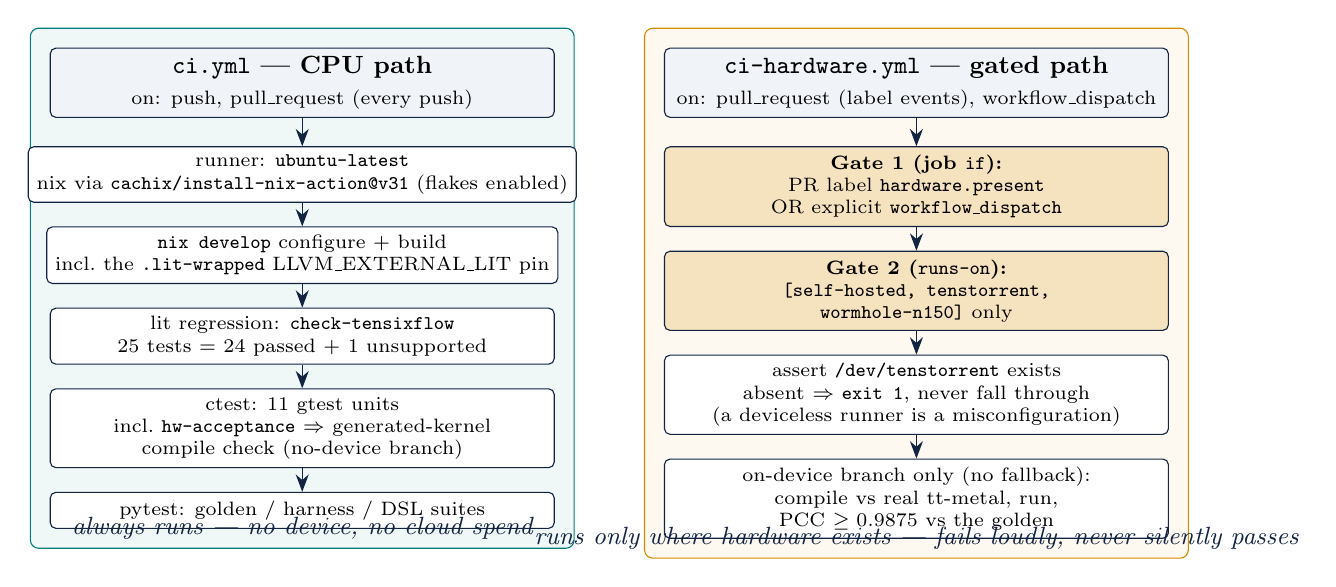
\begin{tikzpicture}[
      box/.style={draw=tensixnavy, rounded corners=2pt, align=center,
                  font=\scriptsize, inner sep=3pt, fill=white,
                  minimum width=6.4cm},
      gate/.style={box, fill=tensixamber!25},
      ok/.style={box, fill=tensixteal!15},
      head/.style={box, fill=tensixlight, font=\small},
      arr/.style={-{Stealth[length=2.2mm]}, tensixnavy},
      paneltitle/.style={font=\small\itshape, tensixnavy},
    ]
    % ---- left: CPU path --------------------------------------------------------
    \node[head] (c0) at (-3.9,0) {\textbf{\texttt{ci.yml} --- CPU path}\\
      \scriptsize on: push, pull\_request (every push)};
    \node[box, below=0.36cm of c0] (c1) {runner: \texttt{ubuntu-latest}\\
      nix via \texttt{cachix/install-nix-action@v31} (flakes enabled)};
    \node[box, below=0.3cm of c1] (c2) {\texttt{nix develop} configure + build\\
      \scriptsize incl.\ the \texttt{.lit-wrapped} LLVM\_EXTERNAL\_LIT pin};
    \node[box, below=0.3cm of c2] (c3) {lit regression: \texttt{check-tensixflow}\\
      \scriptsize 25 tests = 24 passed + 1 unsupported};
    \node[box, below=0.3cm of c3] (c4) {ctest: 11 gtest units\\
      \scriptsize incl.\ \texttt{hw-acceptance} $\Rightarrow$ generated-kernel\\
      \scriptsize compile check (no-device branch)};
    \node[box, below=0.3cm of c4] (c5) {pytest: golden / harness / DSL suites};
    \draw[arr] (c0) -- (c1); \draw[arr] (c1) -- (c2); \draw[arr] (c2) -- (c3);
    \draw[arr] (c3) -- (c4); \draw[arr] (c4) -- (c5);
    \begin{scope}[on background layer]
      \node[fit=(c0)(c5), draw=tensixteal, rounded corners=3pt,
            fill=tensixteal!6, inner sep=7pt] (cpupanel) {};
    \end{scope}
    \node[paneltitle, anchor=south] at (cpupanel.south)
      {always runs --- no device, no cloud spend};

    % ---- right: gated hardware path ---------------------------------------------
    \node[head] (h0) at (3.9,0) {\textbf{\texttt{ci-hardware.yml} --- gated path}\\
      \scriptsize on: pull\_request (label events), workflow\_dispatch};
    \node[gate, below=0.36cm of h0] (h1) {\textbf{Gate 1 (job \texttt{if}):}\\
      PR label \texttt{hardware.present}\\ OR explicit \texttt{workflow\_dispatch}};
    \node[gate, below=0.3cm of h1] (h2) {\textbf{Gate 2 (\texttt{runs-on}):}\\
      \texttt{[self-hosted, tenstorrent,}\\ \texttt{wormhole-n150]} only};
    \node[box, below=0.3cm of h2] (h3) {assert \texttt{/dev/tenstorrent} exists\\
      \scriptsize absent $\Rightarrow$ \texttt{exit 1}, never fall through\\
      \scriptsize (a deviceless runner is a misconfiguration)};
    \node[box, below=0.3cm of h3] (h4) {on-device branch only (no fallback):\\
      \scriptsize compile vs real tt-metal, run,\\
      \scriptsize PCC $\ge 0.9875$ vs the golden};
    \draw[arr] (h0) -- (h1); \draw[arr] (h1) -- (h2); \draw[arr] (h2) -- (h3);
    \draw[arr] (h3) -- (h4);
    \begin{scope}[on background layer]
      \node[fit=(h0)(h4), draw=tensixamber, rounded corners=3pt,
            fill=tensixamber!6, inner sep=7pt] (hwpanel) {};
    \end{scope}
    \node[paneltitle, anchor=south] at (hwpanel.south)
      {runs only where hardware exists --- fails loudly, never silently passes};
  \end{tikzpicture}
  \caption{CI topology: the CPU path (\texttt{ci.yml}) runs the full
  build/lit/ctest/pytest chain on every push, with the generated-kernel
  compile check riding inside ctest's \texttt{hw-acceptance} test; the
  hardware path (\texttt{ci-hardware.yml}) is double-gated
  (Section~\ref{sec:hardware-acceptance}) and only ever runs on a tagged
  self-hosted runner carrying the device.}
  \label{fig:deploy-ci-topology}
\end{figure}

Notes on the CPU path (all from \texttt{.github/workflows/ci.yml}): the
ctest step passes \texttt{--no-tests=ignore} and the pytest step tolerates
exit code 5 (``no tests ran'') so both stayed green in early waves; today
both carry real suites. The generated-kernel compile check is not a separate
CI step --- it is enforced inside ctest via \texttt{hw-acceptance}, whose
no-device branch runs
\path{scripts/hw_bringup_dryrun.sh && cmake --build build --target
check-generated-kernels-compile} (Section~\ref{sec:hardware-acceptance}).

\subsection{Cloud policy: opt-in, documented, never invoked}

The MVP is local-first by policy:
\begin{itemize}[nosep]
  \item \texttt{docs/remote-box.md} states it up front: ``You do not need
        this.'' A remote Linux build box is \emph{purely opt-in}, for keeping
        a laptop free; the document's provider notes (e.g.\ PrimeIntellect
        CPU sandboxes as the cheapest option) are indicative price ordering,
        to be verified in-console.
  \item \texttt{scripts/remote-box.sh} is an idempotent setup script run
        \emph{manually} on a machine the user already owns access to:
        install nix if absent, clone the repo, enter the dev shell, run the
        standard configure + build. It provisions nothing and is never
        invoked by CI.
  \item Nothing in \texttt{ci.yml}, \texttt{ci-hardware.yml}, or the test
        suites provisions or contacts a cloud provider, and nothing incurs
        cloud spend automatically. Likewise \texttt{scripts/build-tt-mlir.sh}
        (the optional tt-mlir study helper) is off the critical path: no
        CMake target depends on it.
\end{itemize}

\subsection{Upstream contribution: scouted, implemented locally, not submitted}

Status, exactly: TensixFlow \emph{scouted} a concrete tt-mlir contribution
and \emph{implemented it locally}; the submission process is fully
documented; and \textbf{nothing was submitted, forked, pushed, or merged}
--- per the project owner's explicit binding instruction. This is policy in
action, not an omission:

\begin{itemize}[nosep]
  \item \textbf{Scouted} (\texttt{docs/upstream\_contribution.md}, todo 58):
        one new lit test for tt-mlir's \texttt{ttir.softmax} verifier,
        covering both error branches --- one of which (shape mismatch) had
        \emph{zero} test coverage anywhere in tt-mlir at the scouted
        revision (\texttt{main} @ \texttt{da6f1ce0}). The gap is cited from
        the actual repo: verifier source, op definition, tree listings, and
        a search over the diagnostic strings.
  \item \textbf{Implemented locally} (\texttt{upstream/tt-mlir/}, todo 59):
        \texttt{softmax\_tests\_negative.mlir} --- 22 lines, three negative
        cases, CHECK strings quoted verbatim from \texttt{SoftmaxOp::verify()}
        --- plus a README recording provenance (scratch clone, \emph{not} a
        fork; branch \texttt{softmax-negative-tests} based on
        \texttt{da6f1ce0}; upstream lint hooks run; scoped diff of exactly
        one new file) and an honest ``what is NOT verified'' section (never
        executed against a real \texttt{ttmlir-opt}, whose toolchain is not
        built on this box).
  \item \textbf{Submission documented, never executed}:
        \texttt{docs/upstream\_contribution.md} records the complete process
        (fork + branch, \texttt{pre-commit}, targeted \texttt{llvm-lit},
        PR template, CI expectations) under a heading that says
        ``DOCUMENTED ONLY; never executed in this plan,'' and states that
        the plan ``explicitly stops before step 1.'' The same constraint is
        repeated in \texttt{upstream/tt-mlir/README.md}.
\end{itemize}

\clearpage
% =============================================================================
% 08_appendix.tex — lane WC
% Sources: .omo/evidence/task-F3-tensixflow.log (F3 final verification wave),
%          docs/hardware_path.md, docs/performance_model.md,
%          kernels/handwritten_baselines/*, .omo/plans glossary terms
% =============================================================================
\section{Appendix}\label{sec:appendix}

\subsection{Verification commands (F3 final wave)}\label{sec:appendix-f3}

Table~\ref{tab:appendix-f3-commands} reproduces the exact command sequence of
the F3 final verification wave
(\path{.omo/evidence/task-F3-tensixflow.log}, 2026-08-03, CPU-only box).
Every step exited 0. The wave additionally recorded: environment probes
confirming \texttt{/dev/tenstorrent} absent and no GPU present; emitted
project contents for both examples (host/reader/compute/writer.cpp +
CMakeLists.txt + README.md); regenerated report artifacts byte-identical to
the committed ones; captured PCC values for both targets on multiple seeds
(all $\ge 0.99998$, floor $0.9875$); and the offline HTML render check under
a network-blocked browser (zero requests, all six section anchors rendered).

\begin{longtable}{@{}p{0.7cm}p{10.6cm}p{3.4cm}@{}}
  \caption{Exact F3 final-wave command sequence with exit codes (all 0).}
  \label{tab:appendix-f3-commands}\\
  \toprule
  \textbf{\#} & \textbf{Exact command} & \textbf{Result (rc)} \\
  \midrule
  \endfirsthead
  \multicolumn{3}{@{}l}{\small\itshape Table \thetable{} (continued)}\\
  \toprule
  \textbf{\#} & \textbf{Exact command} & \textbf{Result (rc)} \\
  \midrule
  \endhead
  \bottomrule
  \endfoot
  1a &
  \begin{minipage}{\linewidth}\begin{lstlisting}
nix develop --command bash -c 'cmake -G Ninja -B build -DMLIR_DIR=$MLIR_DIR -DLLVM_DIR=$LLVM_DIR -DLLVM_EXTERNAL_LIT=$(dirname $(which lit))/.lit-wrapped'
\end{lstlisting}\end{minipage}
  & configure rc=0 (MLIR 20.1.8 pinned) \\
  1b &
  \begin{minipage}{\linewidth}\begin{lstlisting}
nix develop --command bash -c 'cmake --build build'
\end{lstlisting}\end{minipage}
  & build rc=0 \\
  2 &
  \begin{minipage}{\linewidth}\begin{lstlisting}
nix develop --command bash -c 'cmake --build build --target check-tensixflow'
\end{lstlisting}\end{minipage}
  & rc=0; 25 = 24 passed + 1 unsupported \\
  3 &
  \begin{minipage}{\linewidth}\begin{lstlisting}
nix develop --command bash -c 'cd build && ctest --output-on-failure'
\end{lstlisting}\end{minipage}
  & rc=0; 11/11 passed \\
  4 &
  \begin{minipage}{\linewidth}\begin{lstlisting}
uv run --with numpy --with pytest pytest python/tensixflow/tests/ -q
\end{lstlisting}\end{minipage}
  & rc=0; 89 passed \\
  5 &
  \begin{minipage}{\linewidth}\begin{lstlisting}
build/bin/tensixflow-opt --tensixflow-infer-tile-layout --tensixflow-fuse-rmsnorm-matmul --tensixflow-plan-noc-sharding --tensixflow-allocate-circular-buffers --tensixflow-lower-to-ttkernel --tensixflow-emit-metalium=output-dir=<dir> examples/rmsnorm_matmul.mlir
# same command for examples/mlp_block.mlir
\end{lstlisting}\end{minipage}
  & rc=0 both examples; 6 files emitted each \\
  6 &
  \begin{minipage}{\linewidth}\begin{lstlisting}
build/bin/tensixflow-opt --tensixflow-plan-noc-sharding --tensixflow-allocate-circular-buffers examples/rmsnorm_matmul.mlir | build/bin/tensixflow-translate --tensixflow-to-json > reports/rmsnorm_matmul_plan.json
build/bin/tensixflow-report --in reports/rmsnorm_matmul_plan.json --out reports/rmsnorm_matmul_report.html
\end{lstlisting}\end{minipage}
  & rc=0; HTML regenerated byte-identical \\
  7 &
  \begin{minipage}{\linewidth}\begin{lstlisting}
uv run --with numpy --with pytest pytest python/tensixflow/tests/test_correctness.py -v
\end{lstlisting}\end{minipage}
  & rc=0; 11/11; all PCC $\ge 0.9875$, trip-wires hold \\
  8 &
  \begin{minipage}{\linewidth}\begin{lstlisting}
nix develop --command bash -c 'bash scripts/hw_acceptance.sh'
\end{lstlisting}\end{minipage}
  & rc=0; no-device branch: dry-run + 4 generated kernels compile, legacy rejected \\
  9 &
  \begin{minipage}{\linewidth}\begin{lstlisting}
uv run --with playwright python f3_offline_html_check.py
\end{lstlisting}\end{minipage}
  & rc=0; zero network requests, 6/6 anchors rendered \\
\end{longtable}

Steps 1--4 of Table~\ref{tab:appendix-f3-commands} were re-executed for this
report with identical outcomes (lit 25 = 24 + 1 unsupported; ctest 11/11;
pytest 89 --- Section~\ref{sec:software-validation}).

\subsection{Glossary}\label{sec:appendix-glossary}

\begin{longtable}{@{}p{3.4cm}p{11.3cm}@{}}
  \caption{Glossary of TensixFlow terms.}
  \label{tab:appendix-glossary}\\
  \toprule
  \textbf{Term} & \textbf{Definition} \\
  \midrule
  \endfirsthead
  \multicolumn{2}{@{}l}{\small\itshape Table \thetable{} (continued)}\\
  \toprule
  \textbf{Term} & \textbf{Definition} \\
  \midrule
  \endhead
  \bottomrule
  \endfoot
  Circular buffer (CB) & A per-core L1 FIFO of tiles staging data between the reader, compute, and writer tile programs. Sized depth $\times$ \texttt{kTileBytes} (a depth-160 buffer occupies $160 \times 2048 = 327{,}680$ B); indexed per the tt-metal \texttt{tt::CBIndex} convention \texttt{c\_0}\ldots\texttt{c\_31} (default pipeline: in0=\texttt{c\_0}, in1=\texttt{c\_1}, out=\texttt{c\_16}); synchronized via \texttt{cb\_reserve\_back}/\texttt{cb\_push\_back} (producer) and \texttt{cb\_wait\_front}/\texttt{cb\_pop\_front} (consumer). \\
  NoC & Network-on-chip: the Wormhole grid's asynchronous interconnect. TensixFlow plans per-core shard placement and tile movement over it (\texttt{noc\_async\_read}/\texttt{noc\_async\_write}, plus multicast to alleviate DRAM bandwidth contention) and estimates the resulting DRAM traffic in the plan. \\
  PCC & Pearson correlation coefficient. The primary numerical metric comparing a result tensor against the fp32-exact NumPy golden; the acceptance floor is 0.9875 in both the simulator harness and the (gated) on-device branch. \\
  Schedule IR & The tile-level \texttt{tensixflow.sched.*} dialect: a \texttt{sched.kernel} holding reader/compute/writer tile programs built from \texttt{tile\_loop} nests plus CB, NoC, and compute ops. It is the shared contract the emitter prints and the functional simulator executes (Section~\ref{sec:software-architecture}). \\
  Shard & The slice of a tensor assigned to one core's L1 by \texttt{tensixflow-plan-noc-sharding}, placed under the modeled 960 KiB CB/shard budget and routed over the NoC. \\
  Tile & The $32\times32$-element unit of data: bf16 tiles are $32\times32\times2 = 2048$ B. Tiles are the unit of CB depth, NoC moves, and compute ops. \\
  Trip-wire & An empirically calibrated PCC threshold set \emph{above} the good case's observed PCC, so a regression trips the wire before it ever approaches the 0.9875 acceptance floor (\texttt{test\_correctness.py}). \\
  Stub headers & Signature-only mirrors of the tt-metal API surface (\texttt{kernels/handwritten\_baselines/tt\_metal\_stubs/}): correct names and signatures, every body empty, pinned to tt-metal \texttt{@df36cd6}. A compile contract only --- no behavior. \\
  Structural-only validation & Validating generated kernels without execution: golden FileCheck patterns against the current tt-metal API plus the \texttt{-fsyntax-only} compile check against the stubs. Never run on hardware; no hardware numerics claimed. \\
  Disjunctive acceptance & The hardware acceptance policy of Section~\ref{sec:hardware-acceptance}: (on-device run AND PCC $\ge 0.9875$) OR (validated no-device substitute). Wired as an explicit \texttt{if/else}, never \texttt{\&\&\ldots||}, so a present-but-failing device can never be masked by the passing no-device branch. \\
\end{longtable}

\subsection{Deviation register}

Documented deviations from the original plan --- notably the no-device
hardware posture (todo 55's on-device entry point \texttt{SKIPPED}: no
Tenstorrent device is owned) and the deliberately unsubmitted upstream
contribution (todo 60 \texttt{SKIPPED} per explicit user instruction) ---
are recorded with their rationale in the decisions section
(Section~\ref{sec:decisions}). Both are policy-sanctioned: each has a
validated substitute (the no-device branch, which passes; the local
implementation plus submission documentation) rather than a silent gap.
%% INTEGRATOR NOTE: sec:decisions is owned by lane WA; if the reference is
%% still undefined at intermediate compile time, it resolves once lane WA's
%% content lands.


\end{document}
